%% 
%% Copyright 2007-2020 Elsevier Ltd
%% 
%% This file is part of the 'Elsarticle Bundle'.
%% ---------------------------------------------
%% 
%% It may be distributed under the conditions of the LaTeX Project Public
%% License, either version 1.2 of this license or (at your option) any
%% later version.  The latest version of this license is in
%%    http://www.latex-project.org/lppl.txt
%% and version 1.2 or later is part of all distributions of LaTeX
%% version 1999/12/01 or later.
%% 
%% The list of all files belonging to the 'Elsarticle Bundle' is
%% given in the file `manifest.txt'.
%% 
%% Template article for Elsevier's document class `elsarticle'
%% with harvard style bibliographic references

\documentclass[preprint,12pt,authoryear]{elsarticle}

%% Use the option review to obtain double line spacing
%% \documentclass[authoryear,preprint,review,12pt]{elsarticle}

%% Use the options 1p,twocolumn; 3p; 3p,twocolumn; 5p; or 5p,twocolumn
%% for a journal layout:
%\documentclass[final,1p,times,authoryear]{elsarticle}
%% \documentclass[final,1p,times,twocolumn,authoryear]{elsarticle}
% \documentclass[final,3p,times,authoryear]{elsarticle}
%% \documentclass[final,3p,times,twocolumn,authoryear]{elsarticle}
 %\documentclass[final,5p,times,authoryear]{elsarticle}
%% \documentclass[final,5p,times,twocolumn,authoryear]{elsarticle}

%% For including figures, graphicx.sty has been loaded in
%% elsarticle.cls. If you prefer to use the old commands
%% please give \usepackage{epsfig}

%% The amssymb package provides various useful mathematical symbols
\usepackage{amssymb, multirow, subcaption}
\usepackage[utf8]{inputenc}
\usepackage[spanish]{babel}
\graphicspath{ {images/} }

%% The amsthm package provides extended theorem environments
%% \usepackage{amsthm}

%% The lineno packages adds line numbers. Start line numbering with
%% \begin{linenumbers}, end it with \end{linenumbers}. Or switch it on
%% for the whole article with \linenumbers.
%% \usepackage{lineno}

%\journal{Nuclear Physics B}

\begin{document}
	
\begin{frontmatter}

%% Title, authors and addresses

%% use the tnoteref command within \title for footnotes;
%% use the tnotetext command for theassociated footnote;
%% use the fnref command within \author or \affiliation for footnotes;
%% use the fntext command for theassociated footnote;
%% use the corref command within \author for corresponding author footnotes;
%% use the cortext command for theassociated footnote;
%% use the ead command for the email address,
%% and the form \ead[url] for the home page:
%% \title{Title\tnoteref{label1}}
%% \tnotetext[label1]{}
%% \author{Name\corref{cor1}\fnref{label2}}
%% \ead{email address}
%% \ead[url]{home page}
%% \fntext[label2]{}
%% \cortext[cor1]{}
%% \affiliation{organization={},
%%            addressline={}, 
%%            city={},
%%            postcode={}, 
%%            state={},
%%            country={}}
%% \fntext[label3]{}

\title{Optimización de la planificación de servicios: análisis de soluciones}
\date{}

%% use optional labels to link authors explicitly to addresses:
%% \author[label1,label2]{}
%% \affiliation[label1]{organization={},
%%             addressline={},
%%             city={},
%%             postcode={},
%%             state={},
%%             country={}}
%%
%% \affiliation[label2]{organization={},
%%             addressline={},
%%             city={},
%%             postcode={},
%%             state={},
%%             country={}}

\author{Gabriela S\'anchez Yepez}

\affiliation{organization={Posgrado en Ingenier\'ia de Sistemas, Universidad Aut\'onoma de Nuevo Le\'on},%Department and Organization
            addressline={gabriela.sanchezypz@uanl.edu.mx}} 
            %city={},
            %postcode={}, 
            %state={},
           % country={}}

\begin{abstract}
%% Text of abstract
Se han propuesto dos modelos para resolver un problema de toma de decisiones. En objetivo del presente trabajo es aplicar herramientas estadísticas que ayuden a determinar si hay diferencias significativas entre las soluciones que proporcionan ambos modelos. 
\end{abstract}

%%Graphical abstract
%\begin{graphicalabstract}
%\includegraphics{grabs}
%\end{graphicalabstract}

%%Research highlights
%\begin{highlights}
%\item Research highlight 1
%\item Research highlight 2
%\end{highlights}

\begin{keyword}
%% keywords here, in the form: keyword \sep keyword

Modelo matemático \sep GRASP reactivo \sep gap

\end{keyword}

\end{frontmatter}

%% \linenumbers

%% main text
\section{Introducci\'on}
\label{intro}

En el presente trabajo se analizan los resultados obtenidos al resolver un problema de planificación de servicios de telecomunicaciones que consiste en asignar órdenes de servicio a un conjunto de cuadrillas de trabajadores, así como en determinar la secuencia en que deben realizarse dichos servicios, con el fin de balancear
el salario de las cuadrillas sujeto a diversas restricciones. Cada orden tiene asignado un puntaje que depende de la dificultad de la misma, por este motivo el salario de los trabajadores depende directamente de la cantidad y el tipo de servicio que realicen.

Ya que no existe una única forma de plantear el balance del salario se proponen dos formulaciones matemáticas. Una de ellas aborda el balance maximizando el mínimo puntaje colectado por las cuadrillas ($s_{min}$), por lo tanto se referirá a esta formulación como modelo {\em Max-Min}. La segunda formulación toma como base el caso ideal, que consiste en considerar que todas las cuadrillas obtienen un puntaje igual a la media de los puntos de las órdenes ($\mu$). Ésta busca que los puntajes colectados por las cuadrillas se alejen lo menos posible de esta media. Es decir, el segundo modelo, al cual se referirá como modelo {\em Min-Max} tiene como función objetivo minimizar la máxima de las desviaciones respecto a $\mu$. Más detalles acerca del problema así como las formulaciones completas se encuentran en el trabajo de \citet{tesis}.


%Sin embargo, es importante resaltar que por la duración de la jornada laboral así como otras restricciones es posible que no siempre se cumpla con la demanda.
%
%La segunda formulación busca minimizar la máxima desviación respecto a la media de puntajes si todas las órdenes fueran realizadas: 
%
%%tal como lo expresa la ecuación \ref{obj1}
%%\begin{equation}
%%\textup{max} \quad s_{min} \label{obj1}.
%%\end{equation}
%Se referirá a este modelo como {\em Max-Min}. La segunda formulación busca minimizar la máxima desviación respecto a la media de puntajes si todas las órdenes fueran realizadas:
%\begin{equation}
%\textup{min} \quad d_{max}, \label{obj2}
%\end{equation}
%donde
%\begin{equation}
%\mu = \frac{1}{m} \displaystyle \sum_{i=1}^{n-1} s_i.
%\label{mediaA}
%\end{equation} 

%toma de decisiones modelado con dos formulaciones matemáticas. Estas formulaciones fueron previamente validadas mediante el optimizador CPLEX versión 12.8 usando un solo hilo. La validación considera dos criterios de paro: un tiempo de cómputo máximo de 7200 segundos o un gap de 0.0\%. La principal diferencia entre estos modelos es la función objetivo, uno de ellos busca maximizar un valor mínimo, mientras que el otro busca minimizar un valor máximo. Para poder distinguir entre las soluciones de los mismos, se referirá al primer modelo como {\em Max-Min} y al segundo como {\em Min-Max}.  

El objetivo del proyecto es determinar si al resolver ambos modelos utilizando como método de solución una metaheurística basada en un GRASP reactivo \citep{tesis}, hay diferencias significativas entre las soluciones. Para cumplir con dicho objetivo se emplean distintos test estadísticos para los cuales se ha seleccionado un nivel de significancia de 0.05.

El resto del documento se distribuye de la siguiente manera: en la sección \ref{datos} se describe cómo se obtienen los datos a analizar, la sección \ref{ed} presenta y analiza los datos utilizando distintas herramientas de estadística descriptiva, mientras que en la sección \ref{pe} se describe el uso de pruebas estadísticas para justificar si hay diferencias entre los datos. Finalmente, la sección \ref{conclusiones} presenta las conclusiones del trabajo.

\section{Datos}
\label{datos}

Se plantean dos formulaciones distintas para resolver un problema de toma de desiciones. Para validar las mismas y contar con un punto de referencia al resolver con la metaheurística GRASP reactiva, los modelos se resuelven con el optimizador CPLEX versión 12.8 usando un solo hilo y considerando dos criterios de paro: un tiempo de cómputo máximo de 7200 segundos o un gap de 0.0\% (soluciones óptimas). 

Las instancias utilizadas en la experimentación son adaptadas de las propuestas en la literatura \citep{chao1996}. El conjunto se divide en siete clases teniendo en total 353 instancias disponibles. Las instancias pertenecientes a una misma clase contienen el mismo grafo y varían en la cantidad de cuadrillas disponibles y tiempo límite para la duración de las rutas. Las características de cada clase de instancias se especifica en el cuadro \ref{instancias}.

\begin{table}
	\centering
	\caption{Instancias.}
	\begin{tabular}{|r|r|r|r|r|r|}
		\hline
		&  & \multicolumn{4}{c|}{\bf Instancias} \\
		\cline{3-6}
		\bf Clase & \bf Órdenes & \multicolumn{3}{c|}{\bf Cuadrillas} & \multirow{2}{1cm}{\bf Total} \\
		\cline{3-5}
		&  & \bf 2 & \bf 3 & \bf 4 & \\
		\hline
		I & 21 & 11 & 11 & 11 & 33 \\
		II & 32 & 17 & 16 & 15 & 48\\
		III & 33 & 20 & 20 & 20 & 60 \\
		IV & 64 & 11 & 8 & 5 & 24 \\
		V & 66 & 25 & 25 & 24 & 74 \\
		VI & 100 & 20 & 19 & 17 & 56 \\
		VII & 102 & 20 & 19 & 19 & 58 \\ 
		\hline
	\end{tabular}
	\label{instancias}
\end{table}

%El GRASP (Greedy Randomized Adaptive Search Procedure) reactivo es una metaheurística multiarranque en la que cada iteración consta de dos fases principales, una fase de construcción y una fase de mejora. La fase de construcción crea una solución que se toma como punto de partida para la fase de mejora. En este caso particular, la fase de mejora consiste en una búsqueda local. El procedimiento se repite un determinado número de iteraciones y se regresa la mejor solución encontrada, es decir, la solución con el mejor valor de la función objetivo.

Debido a la naturaleza aleatoria del GRASP reactivo, se proporcionan diez soluciones a cada instancia para obtener poblaciones de tamaño 3530. Teniendo en mente el punto de referencia, los conjuntos de datos que se analizan son diferencias porcentuales ({\bf gap}) entre el valor objetivo de las soluciones obtenidas con la metaheurística y el valor objetivo de la mejor solución encontrada por CPLEX, para un modelo en particular.

Por ejemplo, el gap para el modelo Max-Min queda determinado por la ecuación (\ref{gap})
\begin{equation}
gap = 100 \times \frac{Z_{\mbox{cplex}} - Z_{\mbox{grasp}}}{Z_{\mbox{cplex}}},
\label{gap}
\end{equation} 
donde $Z_{\mbox{cplex}}$ y $Z_{\mbox{grasp}}$ representan el valor de la funci\'on objetivo obtenida por CPLEX y el GRASP reactivo, respectivamente.

Es claro que el gap puede ser tanto positivo como negativo. Si es positivo indica que el valor objetivo encontrado con CPLEX es mejor que el encontrado por la metaheurística, en cambio si es negativa indica que el valor objetivo encontrado con la metaheurística es mejor que el determinado por el optimizador. Para tener la misma interpretación al analizar los resultados del modelo Min-Max, el gap determinado por ecuación \ref{gap} se multiplica por (-1).
%Se tienen soluciones a dos formulaciones distintas, cada una de ellas tiene un valor objetivo específico. Los valores objetivo de las soluciones que se obtienen al resolver el modelo Max-Min se les identifica como $s_1$, mientras que los valores objetivo de las soluciones obtenidas al resolver el modelo Min-Max se identifican con $s_2$. 

Es de interés determinar el comportamiento que siguen las soluciones obtenidas con un modelo específico al evaluar con una función objetivo distinta. En este caso las soluciones del modelo Max-Min son evaluadas en la función objetivo del modelo Min-Max y las soluciones del modelo Min-Max son evaluadas en la función objetivo del modelo Max-Min. 

Considerando toda la información descrita en la sección, en total se analizan cuatro conjuntos de soluciones: las del modelo Max-Min, las soluciones del modelo Min-Max evaluadas en la función objetivo del modelo Max-Min, las del modelo Min-Max y las soluciones del modelo Max-Min evaluadas en la función objetivo del modelo Min-Max, identificadas por $s_1, s_{21}, s_2$ y $s_{12}$, respectivamente. El cálculo del gap en cada uno de estos conjuntos da lugar a los cuatro distintos conjuntos de datos que se analizan en el trabajo. 

%Con el objetivo de tener el mismo punto de referencia, se calcula la diferencia porcentual entre el valor objetivo de la evaluación de la solución y el valor objetivo de la mejor solución encontrada por CPLEX en el modelo correspondiente. Estas diferencias porcentuales serán las que se analizan en este trabajo.
%Es claro que las diferencias porcentuales pueden ser tanto positivas como negativas. Si la diferencia es positiva indica que el valor objetivo encontrado con CPLEX es mejor que el encontrado por la metaheurística, en cambio si es negativa indica que el valor objetivo encontrado con la metaheurística es mejor que el determinado por el optimizador.
%Debido a la naturaleza aleatoria del método de solución, se proporcionan diez soluciones a cada instancia para obtener poblaciones de tamaño 3530.

\section{Estadística descriptiva}
\label{ed}

%En esta sección se presentan analizan los datos utilizando diversas herramientas gráficas.

La distribución de los resultados del gap en cada conjunto de datos se presentan en las figuras \ref{histob1} y \ref{histob2}. El apoyo visual de estas figuras permite identificar que existe un gran número de replicas para las cuales no hay diferencia entre los dos métodos de solución empleados (metaheurística y optimizador). Esto es de esperarse ya que el optimizador logra encontrar soluciones óptimas para aproximadamente un 50\% del total de las instancias en ambos modelos y los resultados de la metaheurística se mantienen muy similares. De forma muy particular en casi el 100\% de las instancias de las clases I y II, los resultados son los mismos, esto puede observarse más a detalle en los diagramas de caja bigote de las figuras \ref{boxob1} y \ref{boxob2}.

Es importante destacar que en adelante el análisis se realiza por pares ya que el interés es determinar si es que alguno de los modelos da mejores resultados. Recuerde que la diferencia entre las formulaciones radica en la función objetivo. 

Los pares de conjuntos que se analizan son el el gap al evaluar las soluciones del modelo Max-Min en la función objetivo Min-Max ($s_{12}$) junto con el gap de las soluciones $s_1$ y, el gap al evaluar las soluciones del modelo Min-Max en la función objetivo Max-Min $s_{21}$ y el gap de las soluciones $s_{2}$. Si se analizan los diagramas de caja bigote de acuerdo a los pares antes mencionados, se puede observar que los resultados son similares con mayor frecuencia en las clases más pequeñas. La figura \ref{densidad} permite observar las densidades de los resultados separados de acuerdo a la función objetivo. En esta figura son más notorias las similitudes que las diferencias.

\begin{figure}
	\centering
	\begin{subfigure}{\textwidth}
		\centering
		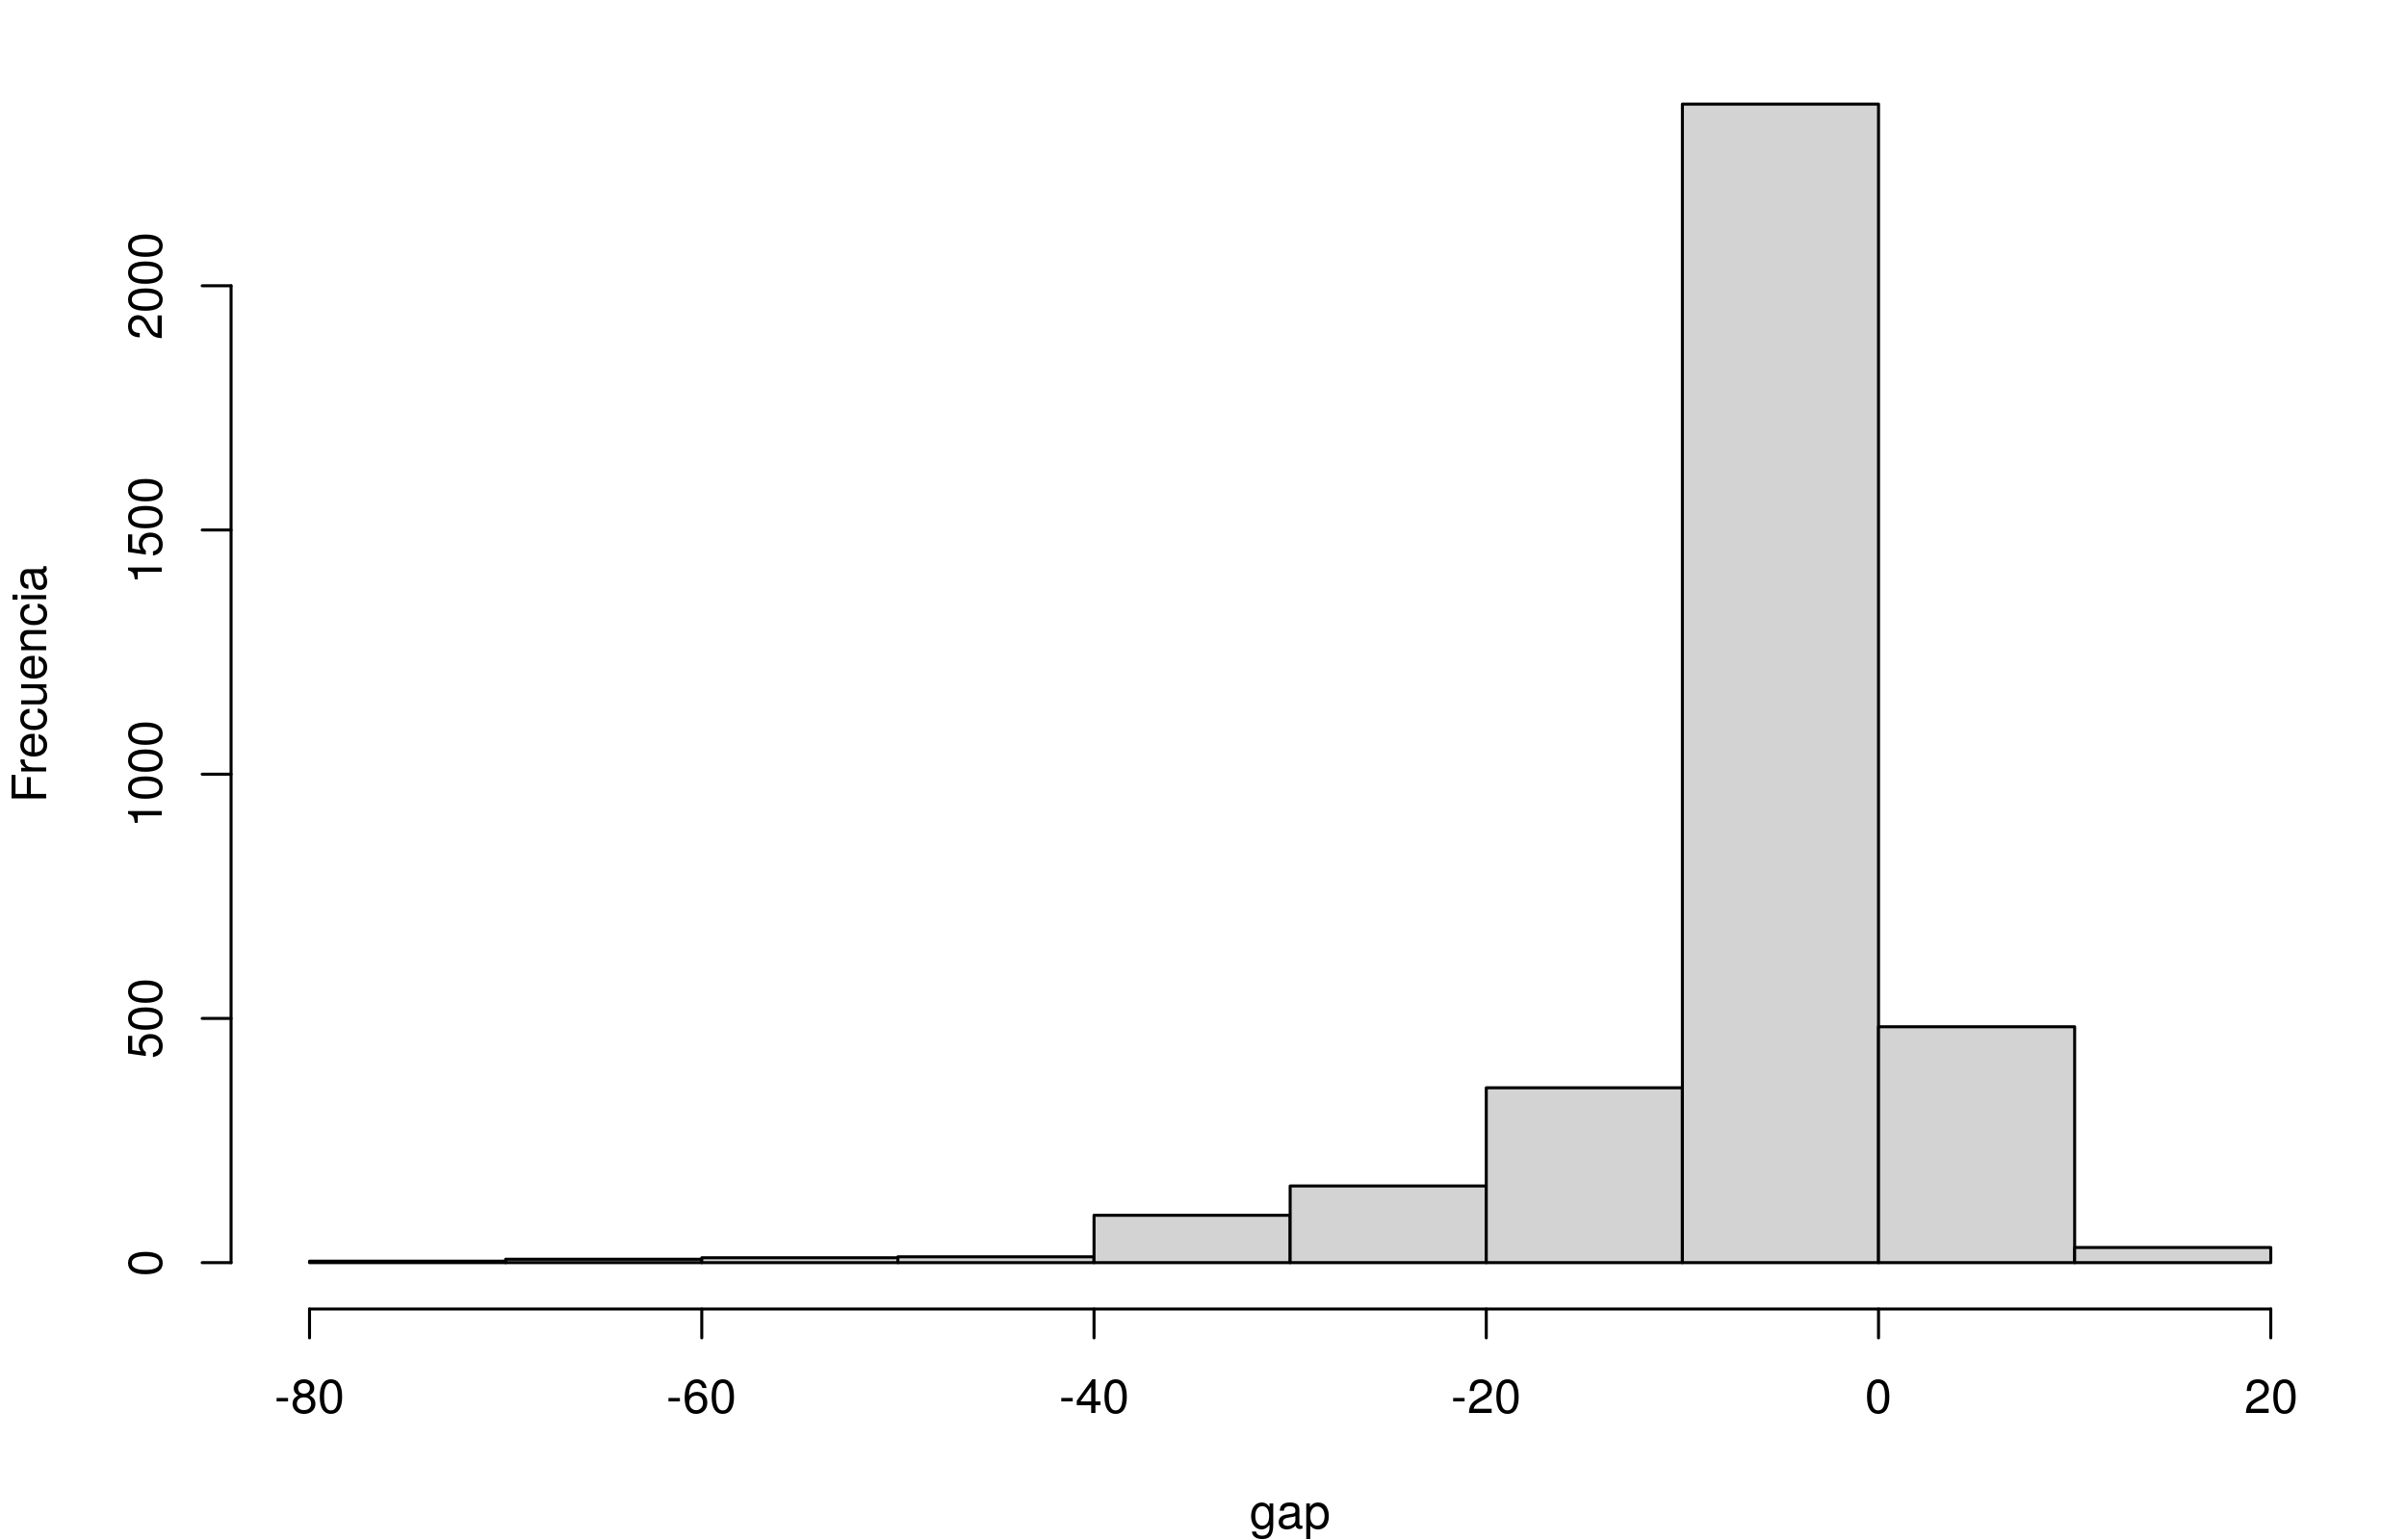
\includegraphics[width=0.8\textwidth]{hist_gap1.png}
		\caption{Soluciones $s_1$}
	\end{subfigure}
	\begin{subfigure}{\textwidth}
		\centering
		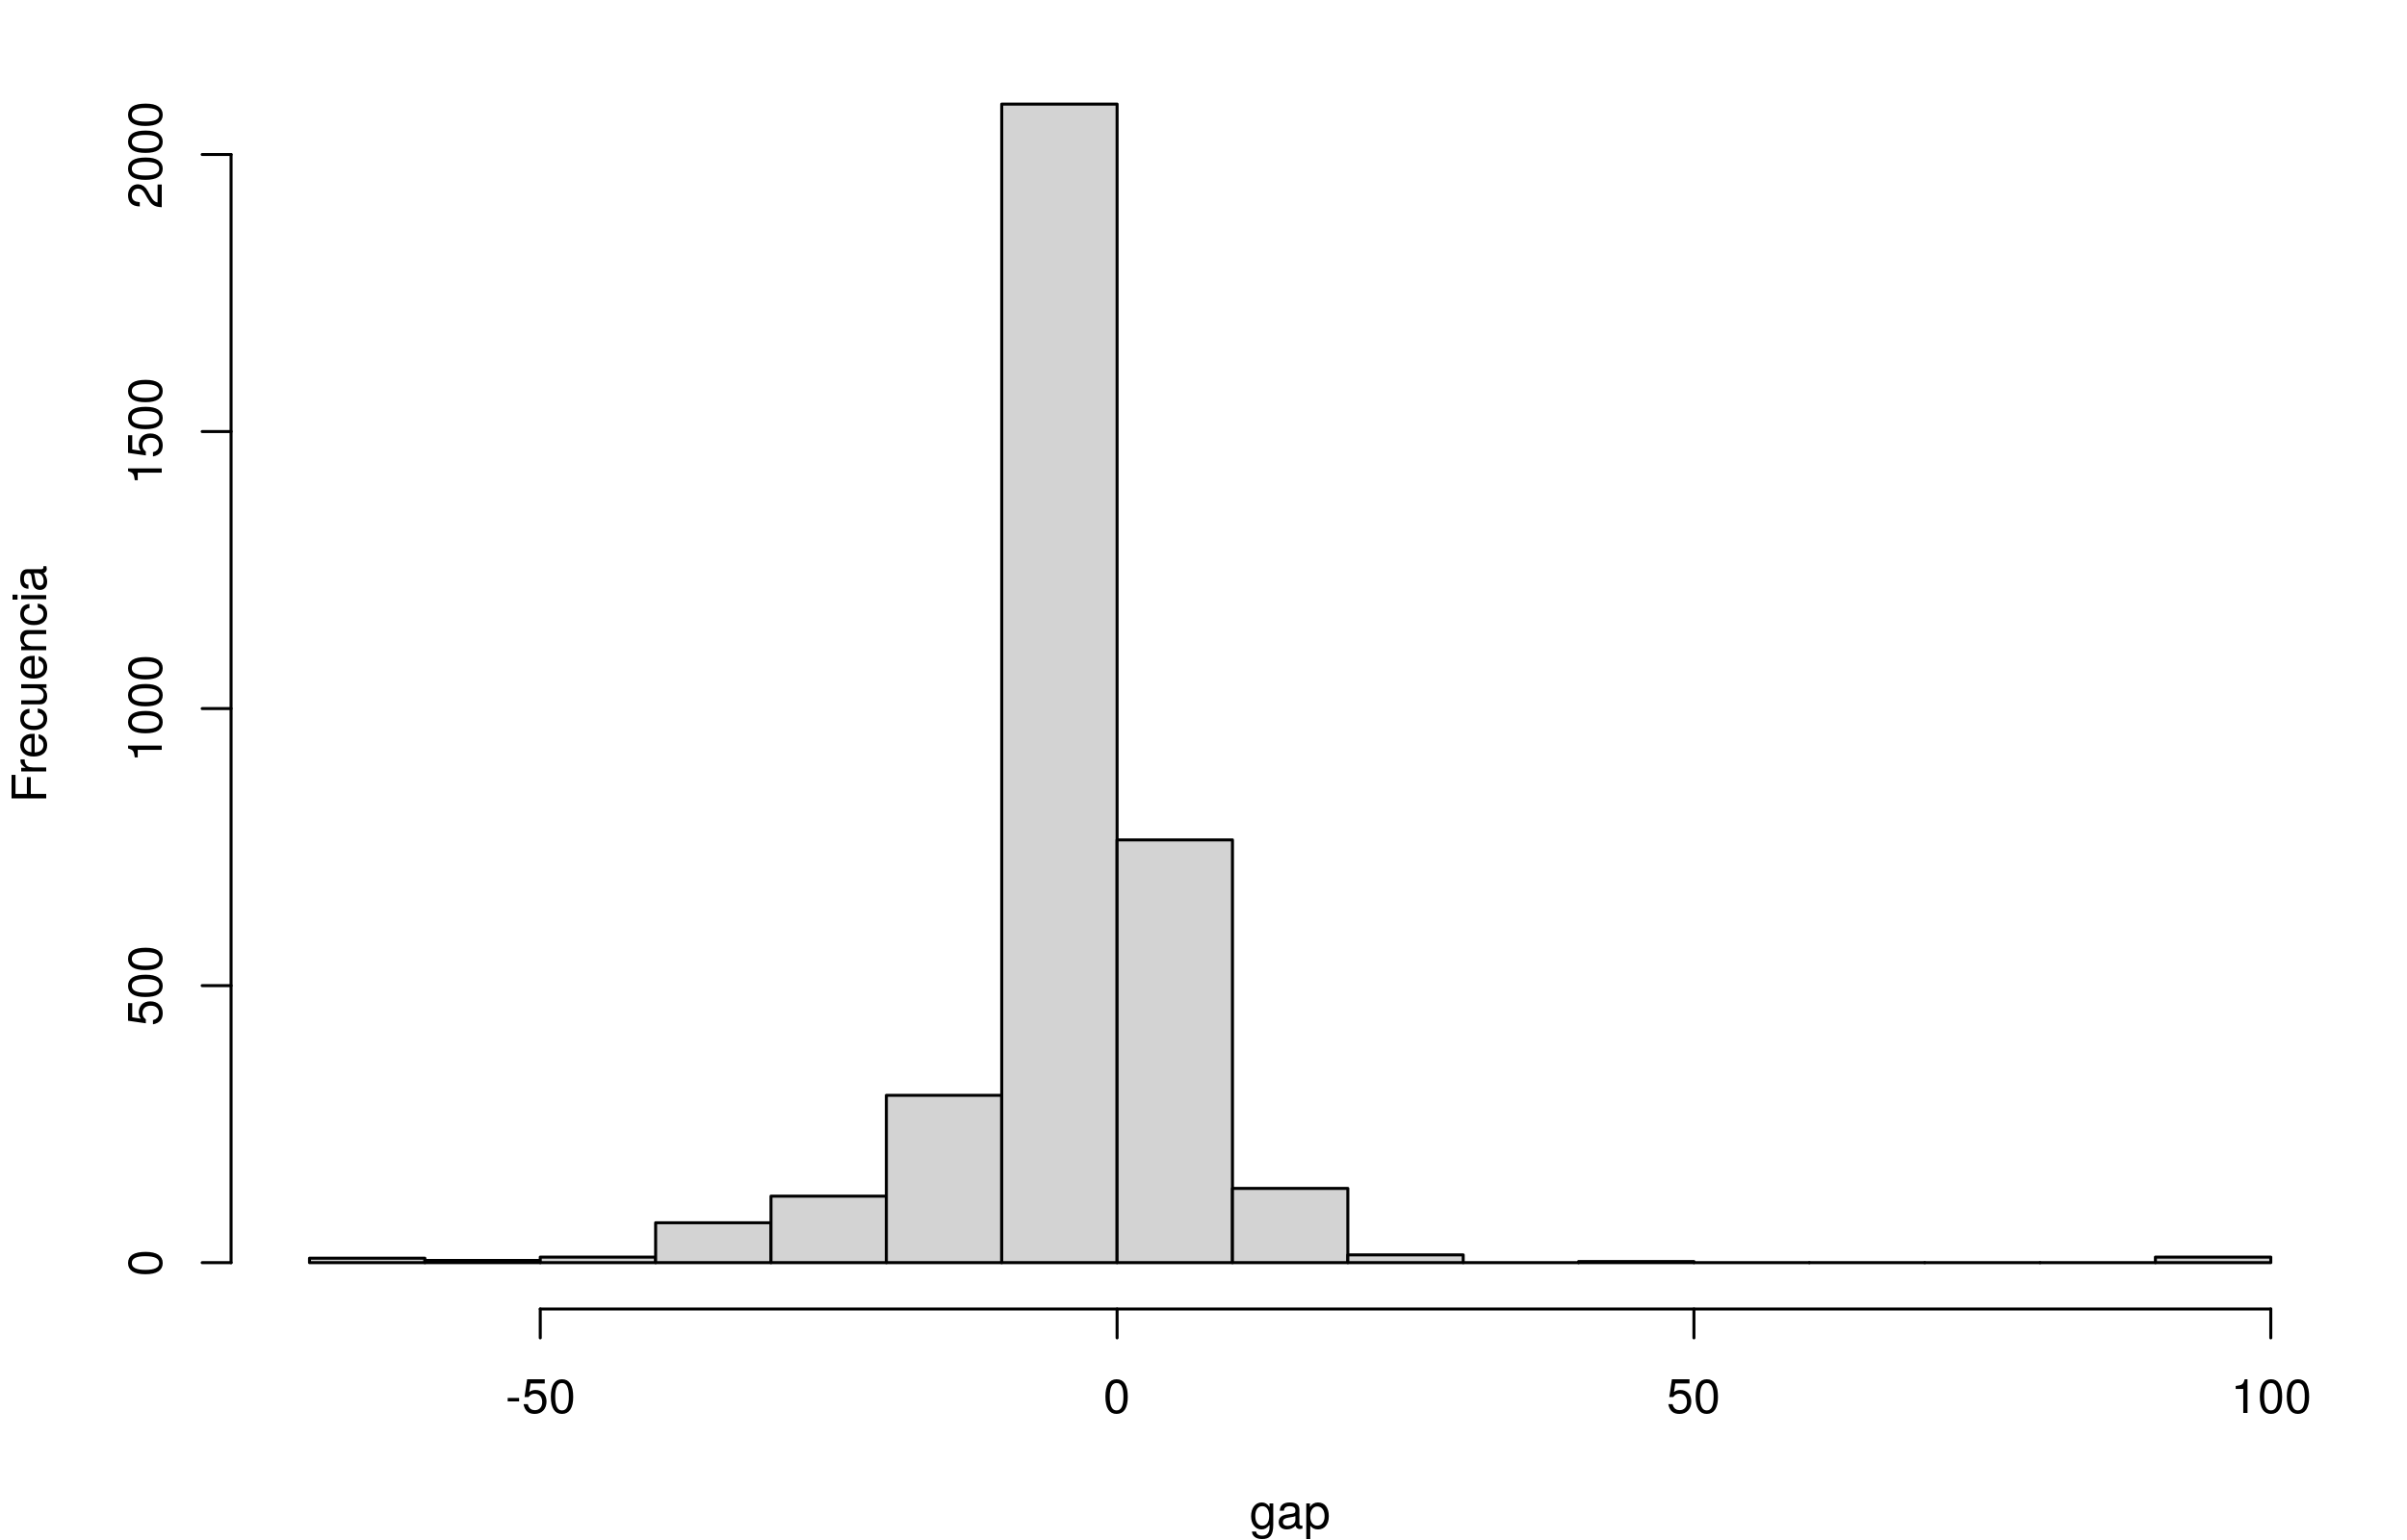
\includegraphics[width=0.8\textwidth]{hist_gap21.png}
		\caption{Soluciones $s_{21}$}
	\end{subfigure}
\caption{Gap para la función objetivo Max-Min.}
\label{histob1}
\end{figure}

\begin{figure}
	\begin{subfigure}{\textwidth}
		\centering
		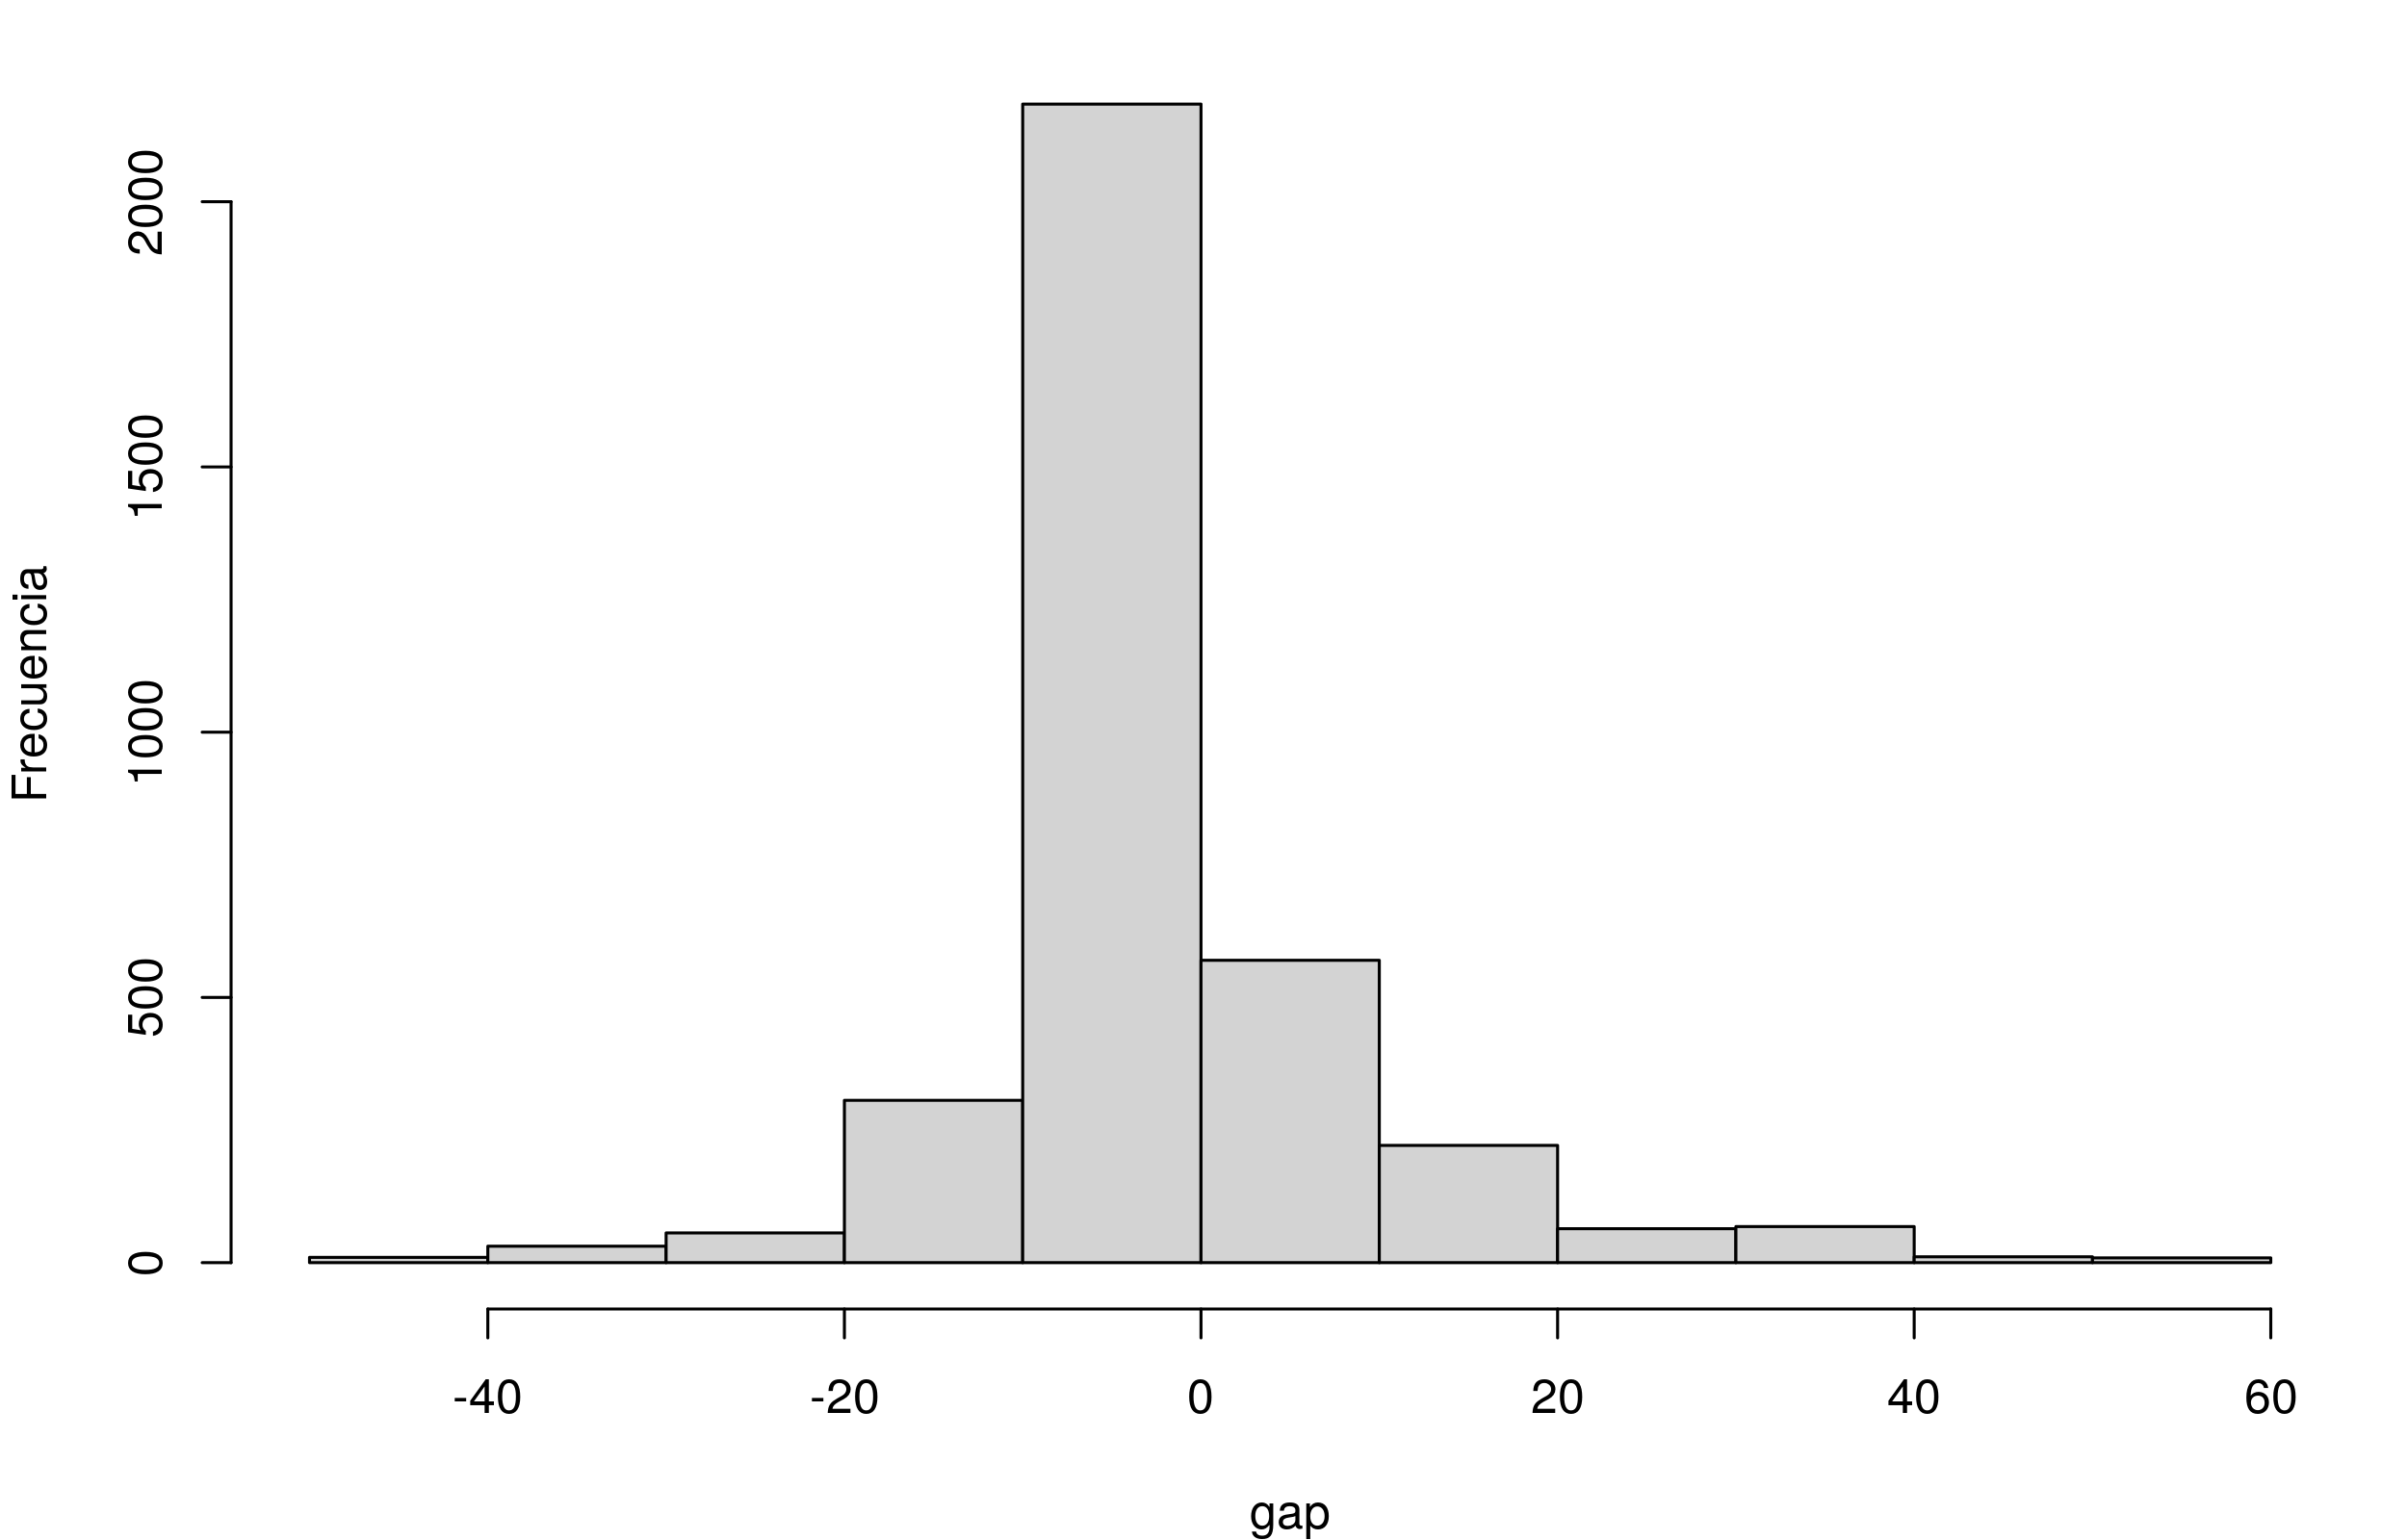
\includegraphics[width=0.8\textwidth]{hist_gap2.png}
		\caption{Soluciones $s_2$}
	\end{subfigure}
	\begin{subfigure}{\textwidth}
		\centering
		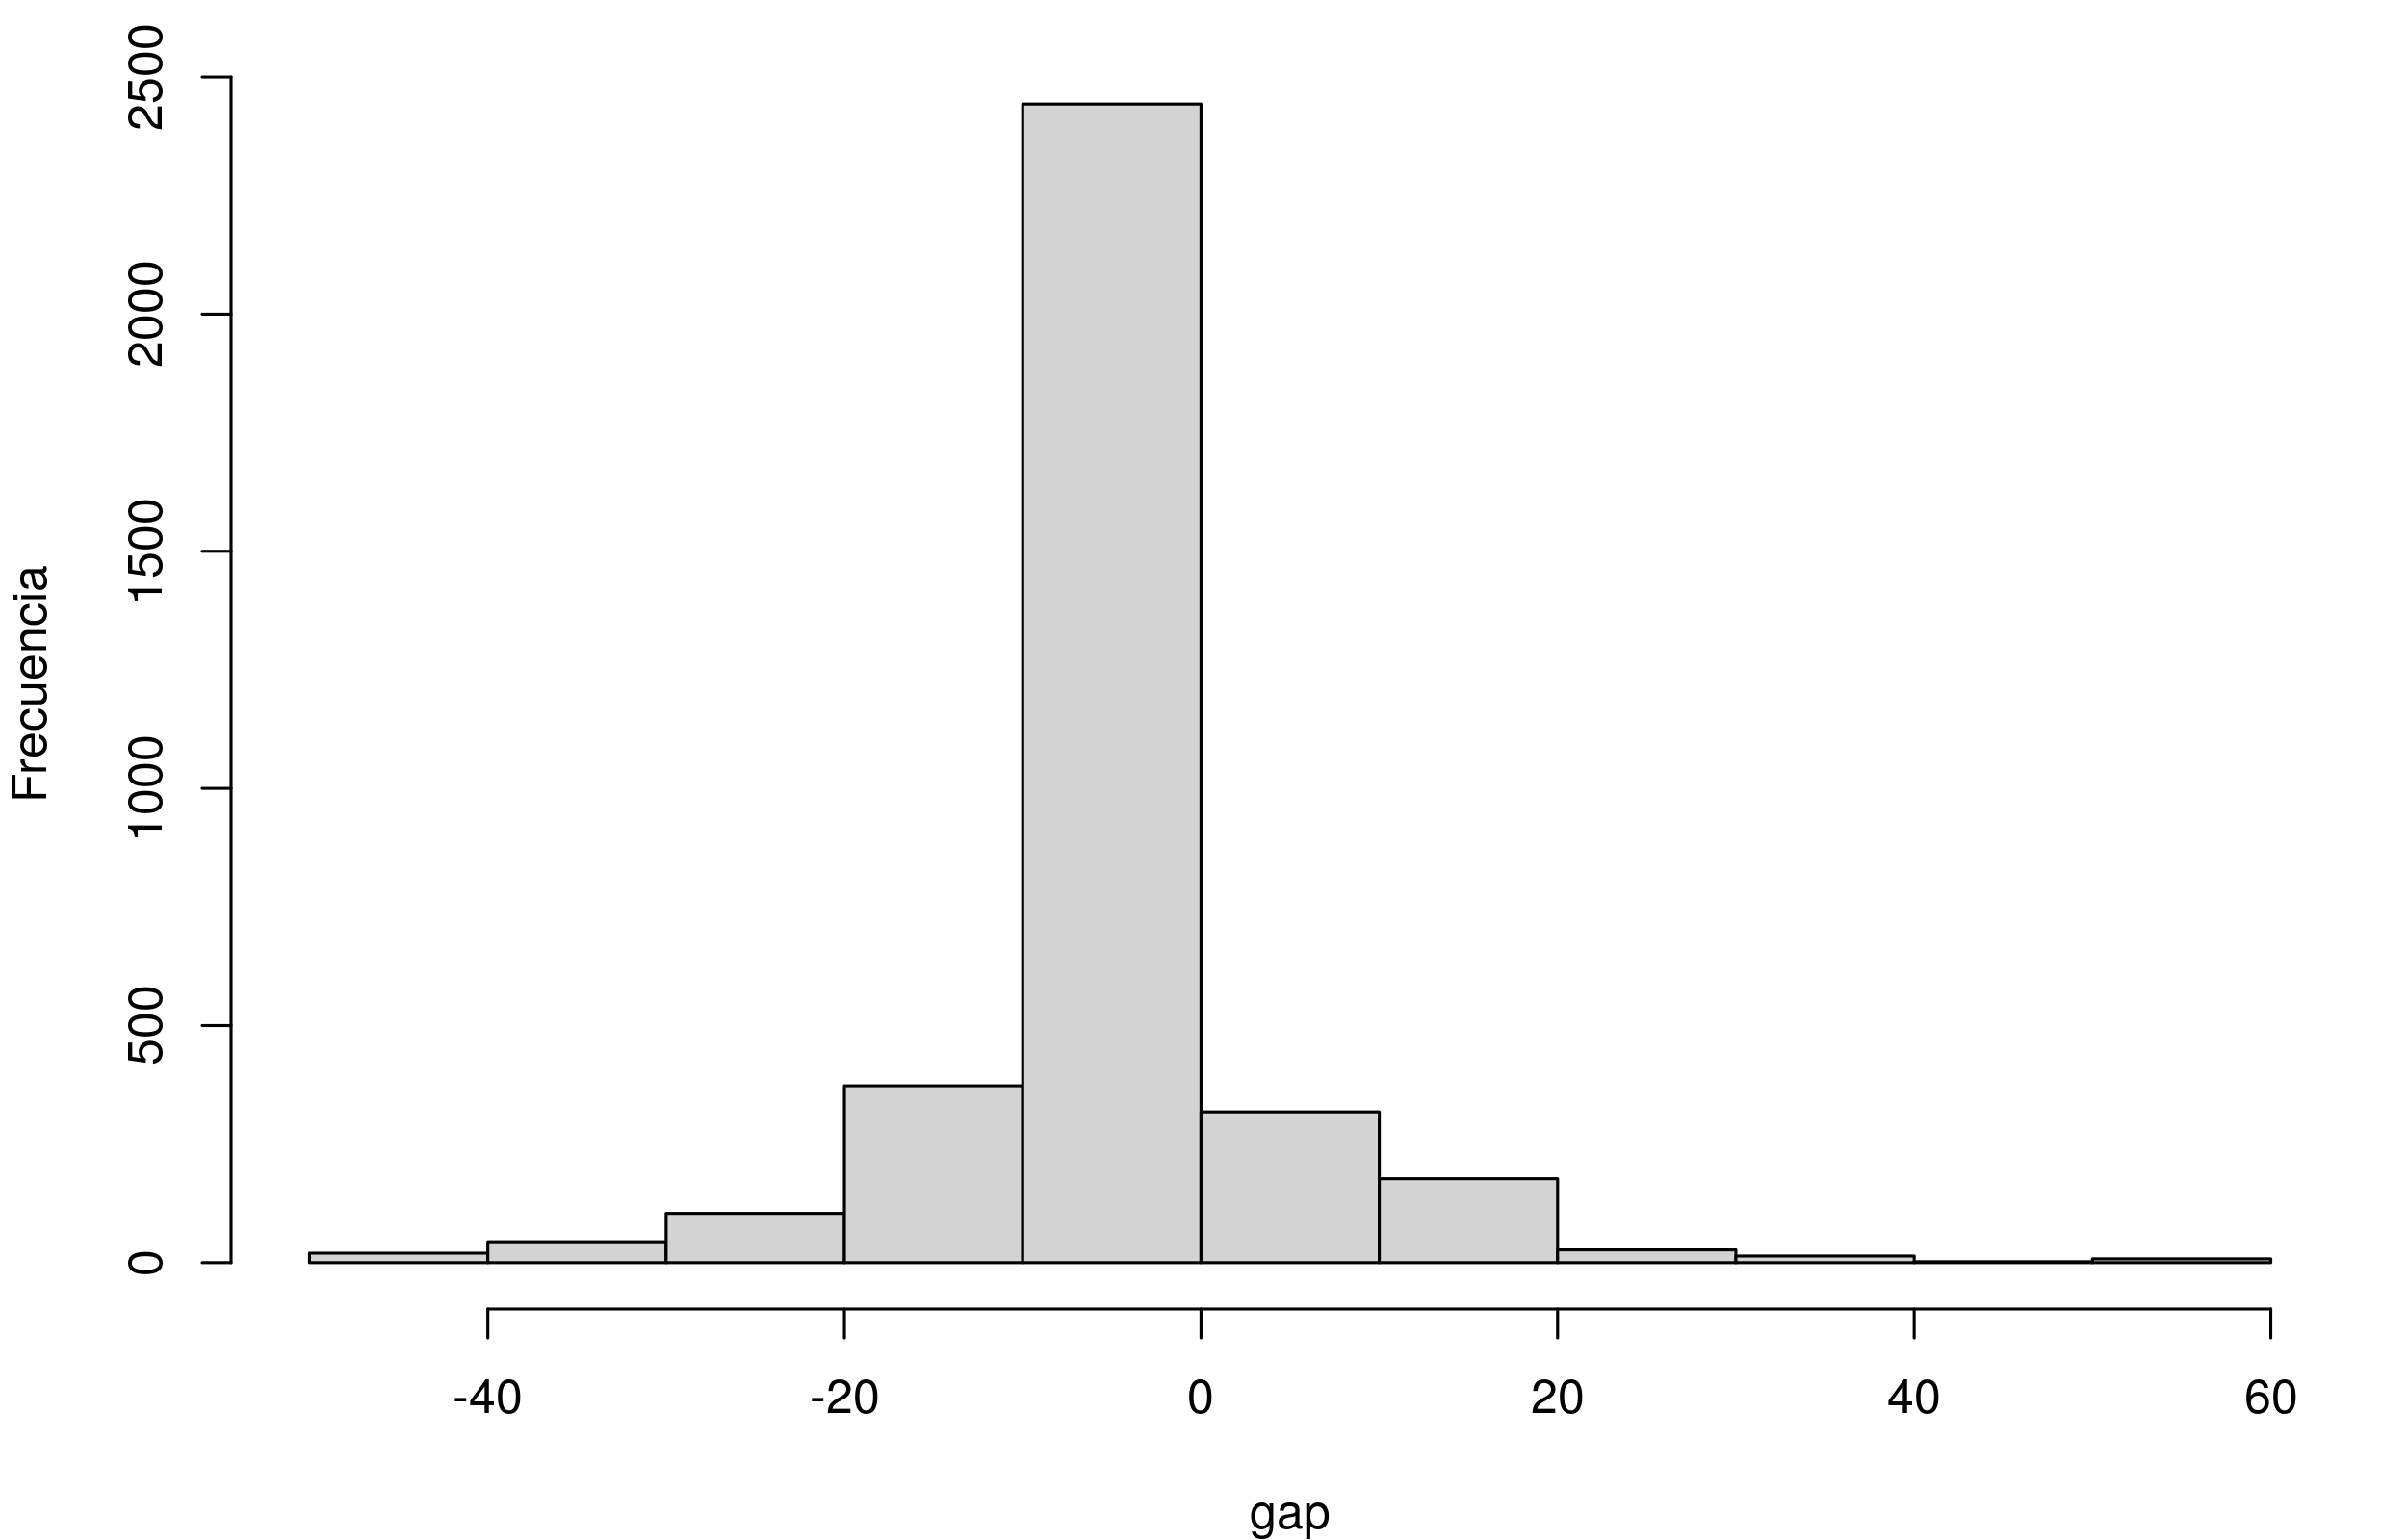
\includegraphics[width=0.8\textwidth]{hist_gap12.png}
		\caption{Soluciones $s_{12}$}
	\end{subfigure}
\caption{Gap para la función objetivo Min-Max.}
\label{histob2}
\end{figure}

\begin{figure}
	\centering
	\begin{subfigure}{\textwidth}
		\centering
		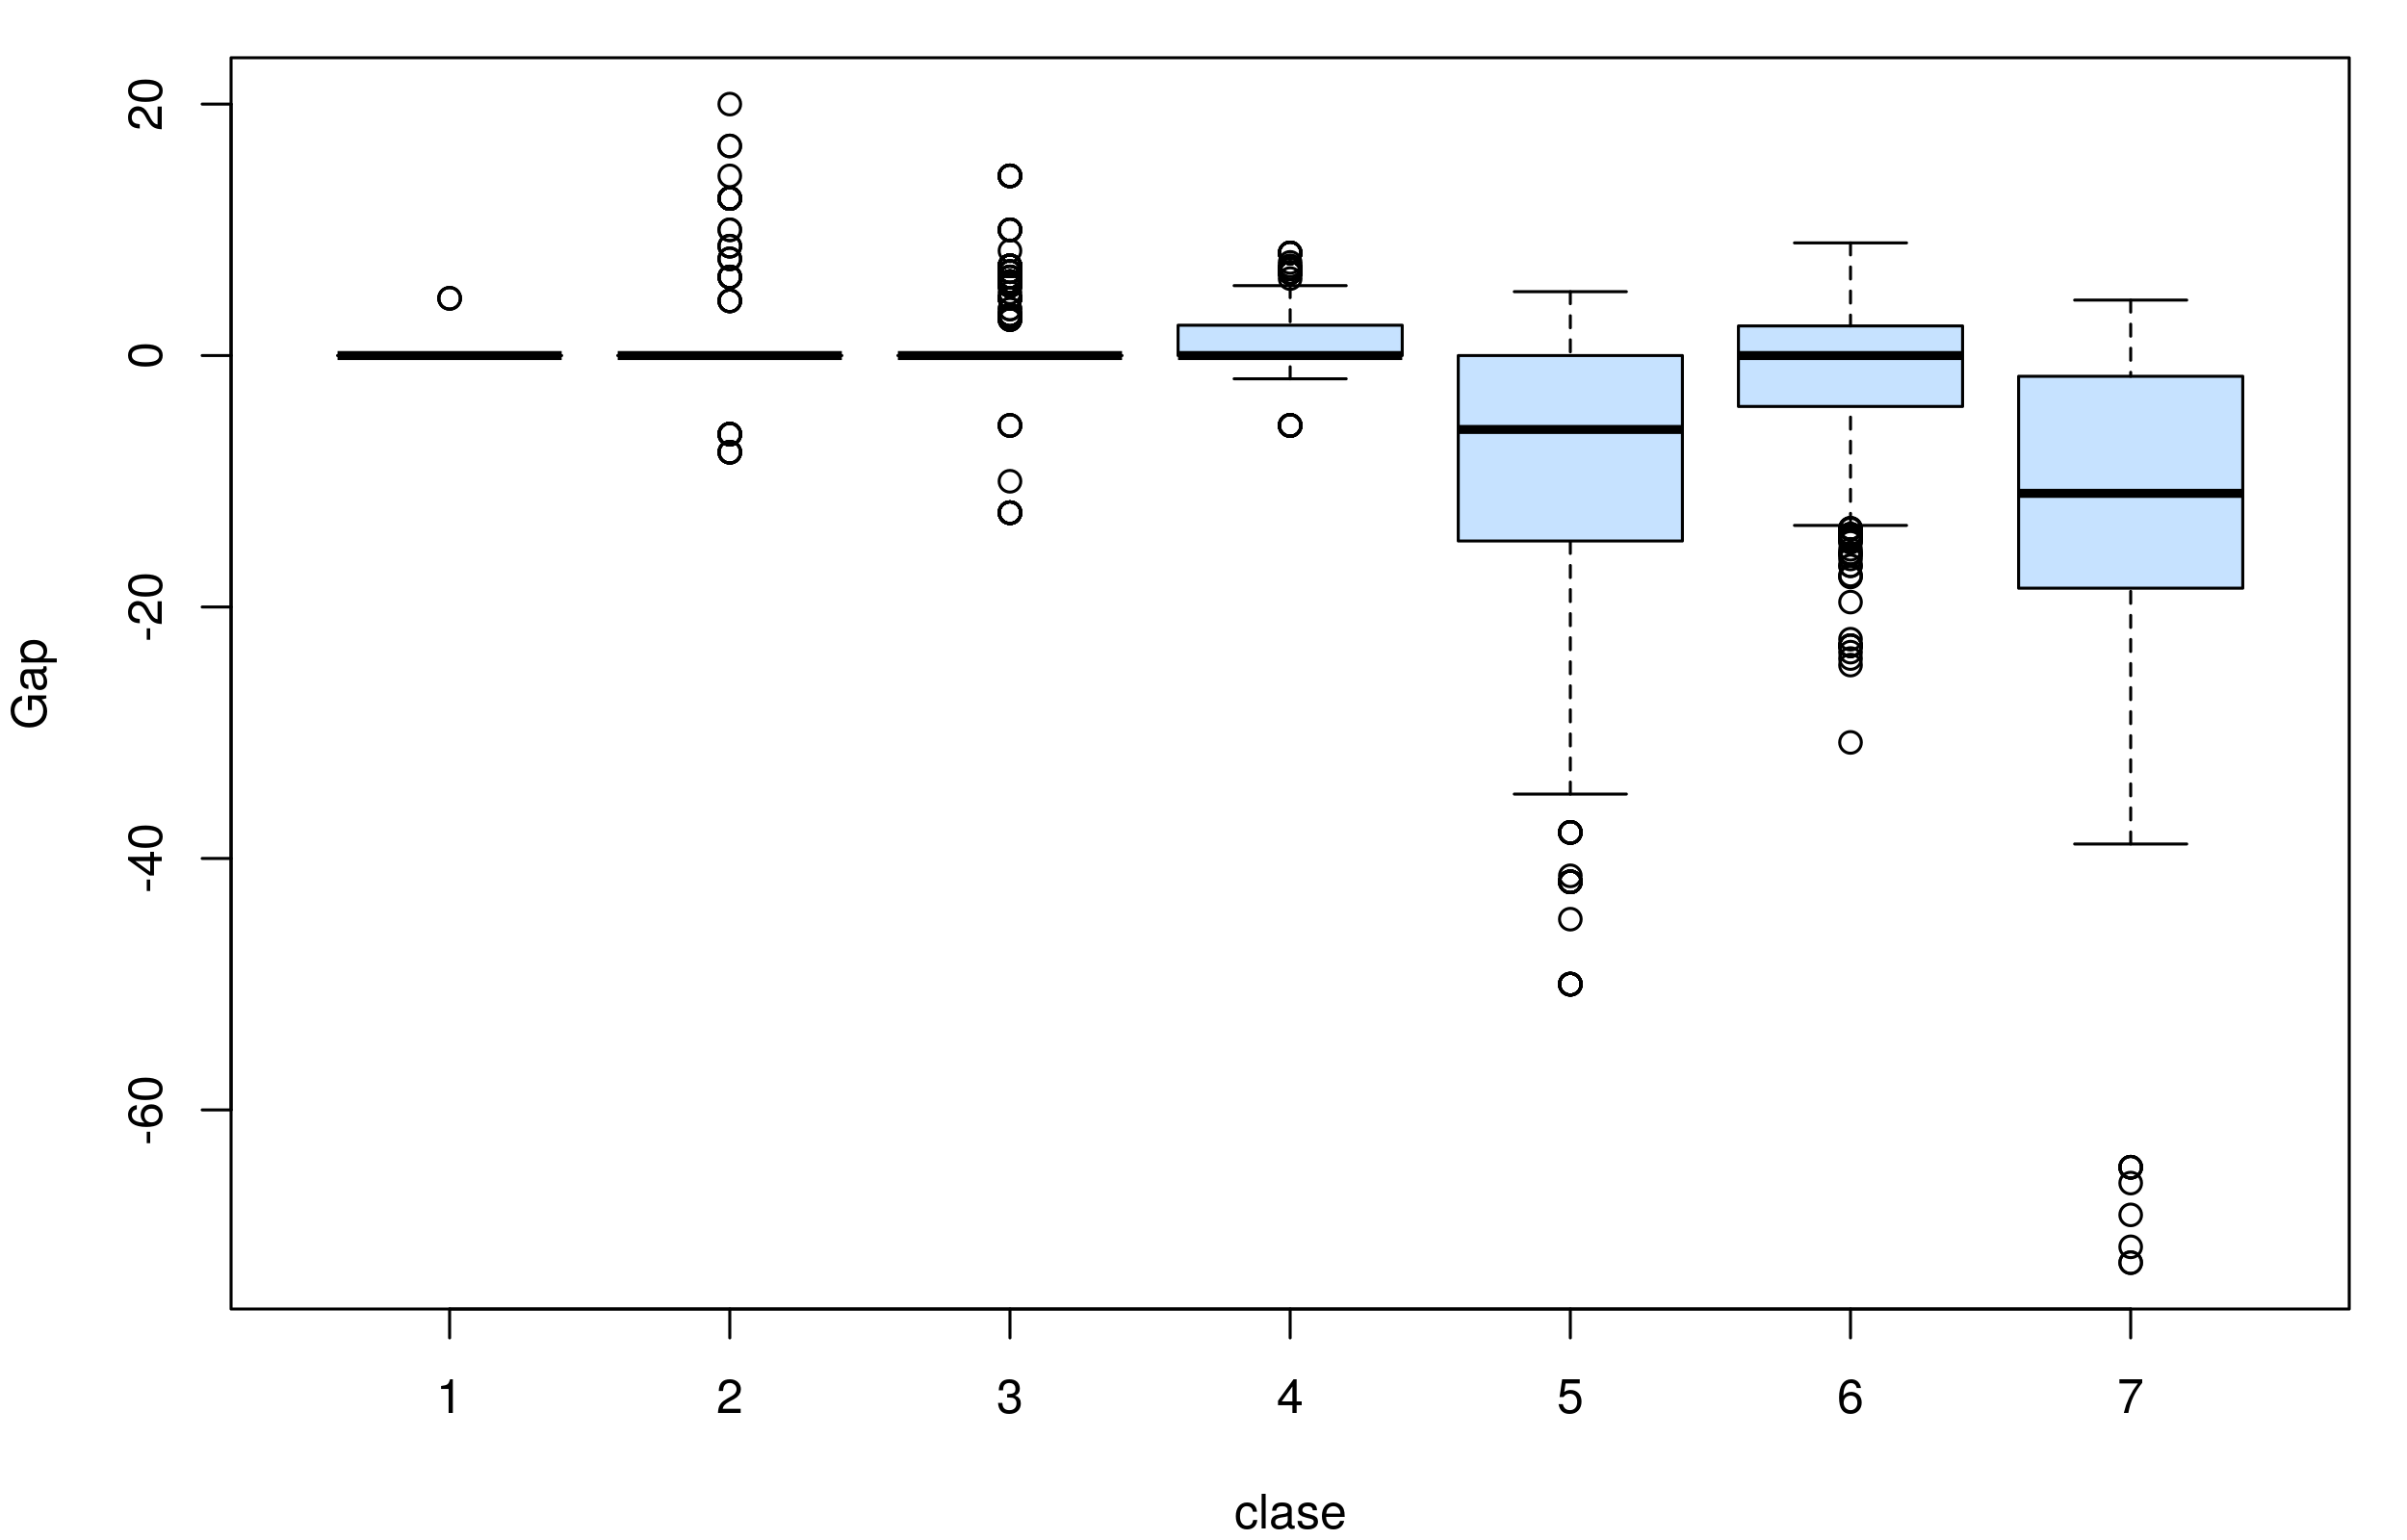
\includegraphics[width=0.8\textwidth]{box_gap1.png}
		\caption{Soluciones $s_1$}
	\end{subfigure}
	\begin{subfigure}{\textwidth}
		\centering
		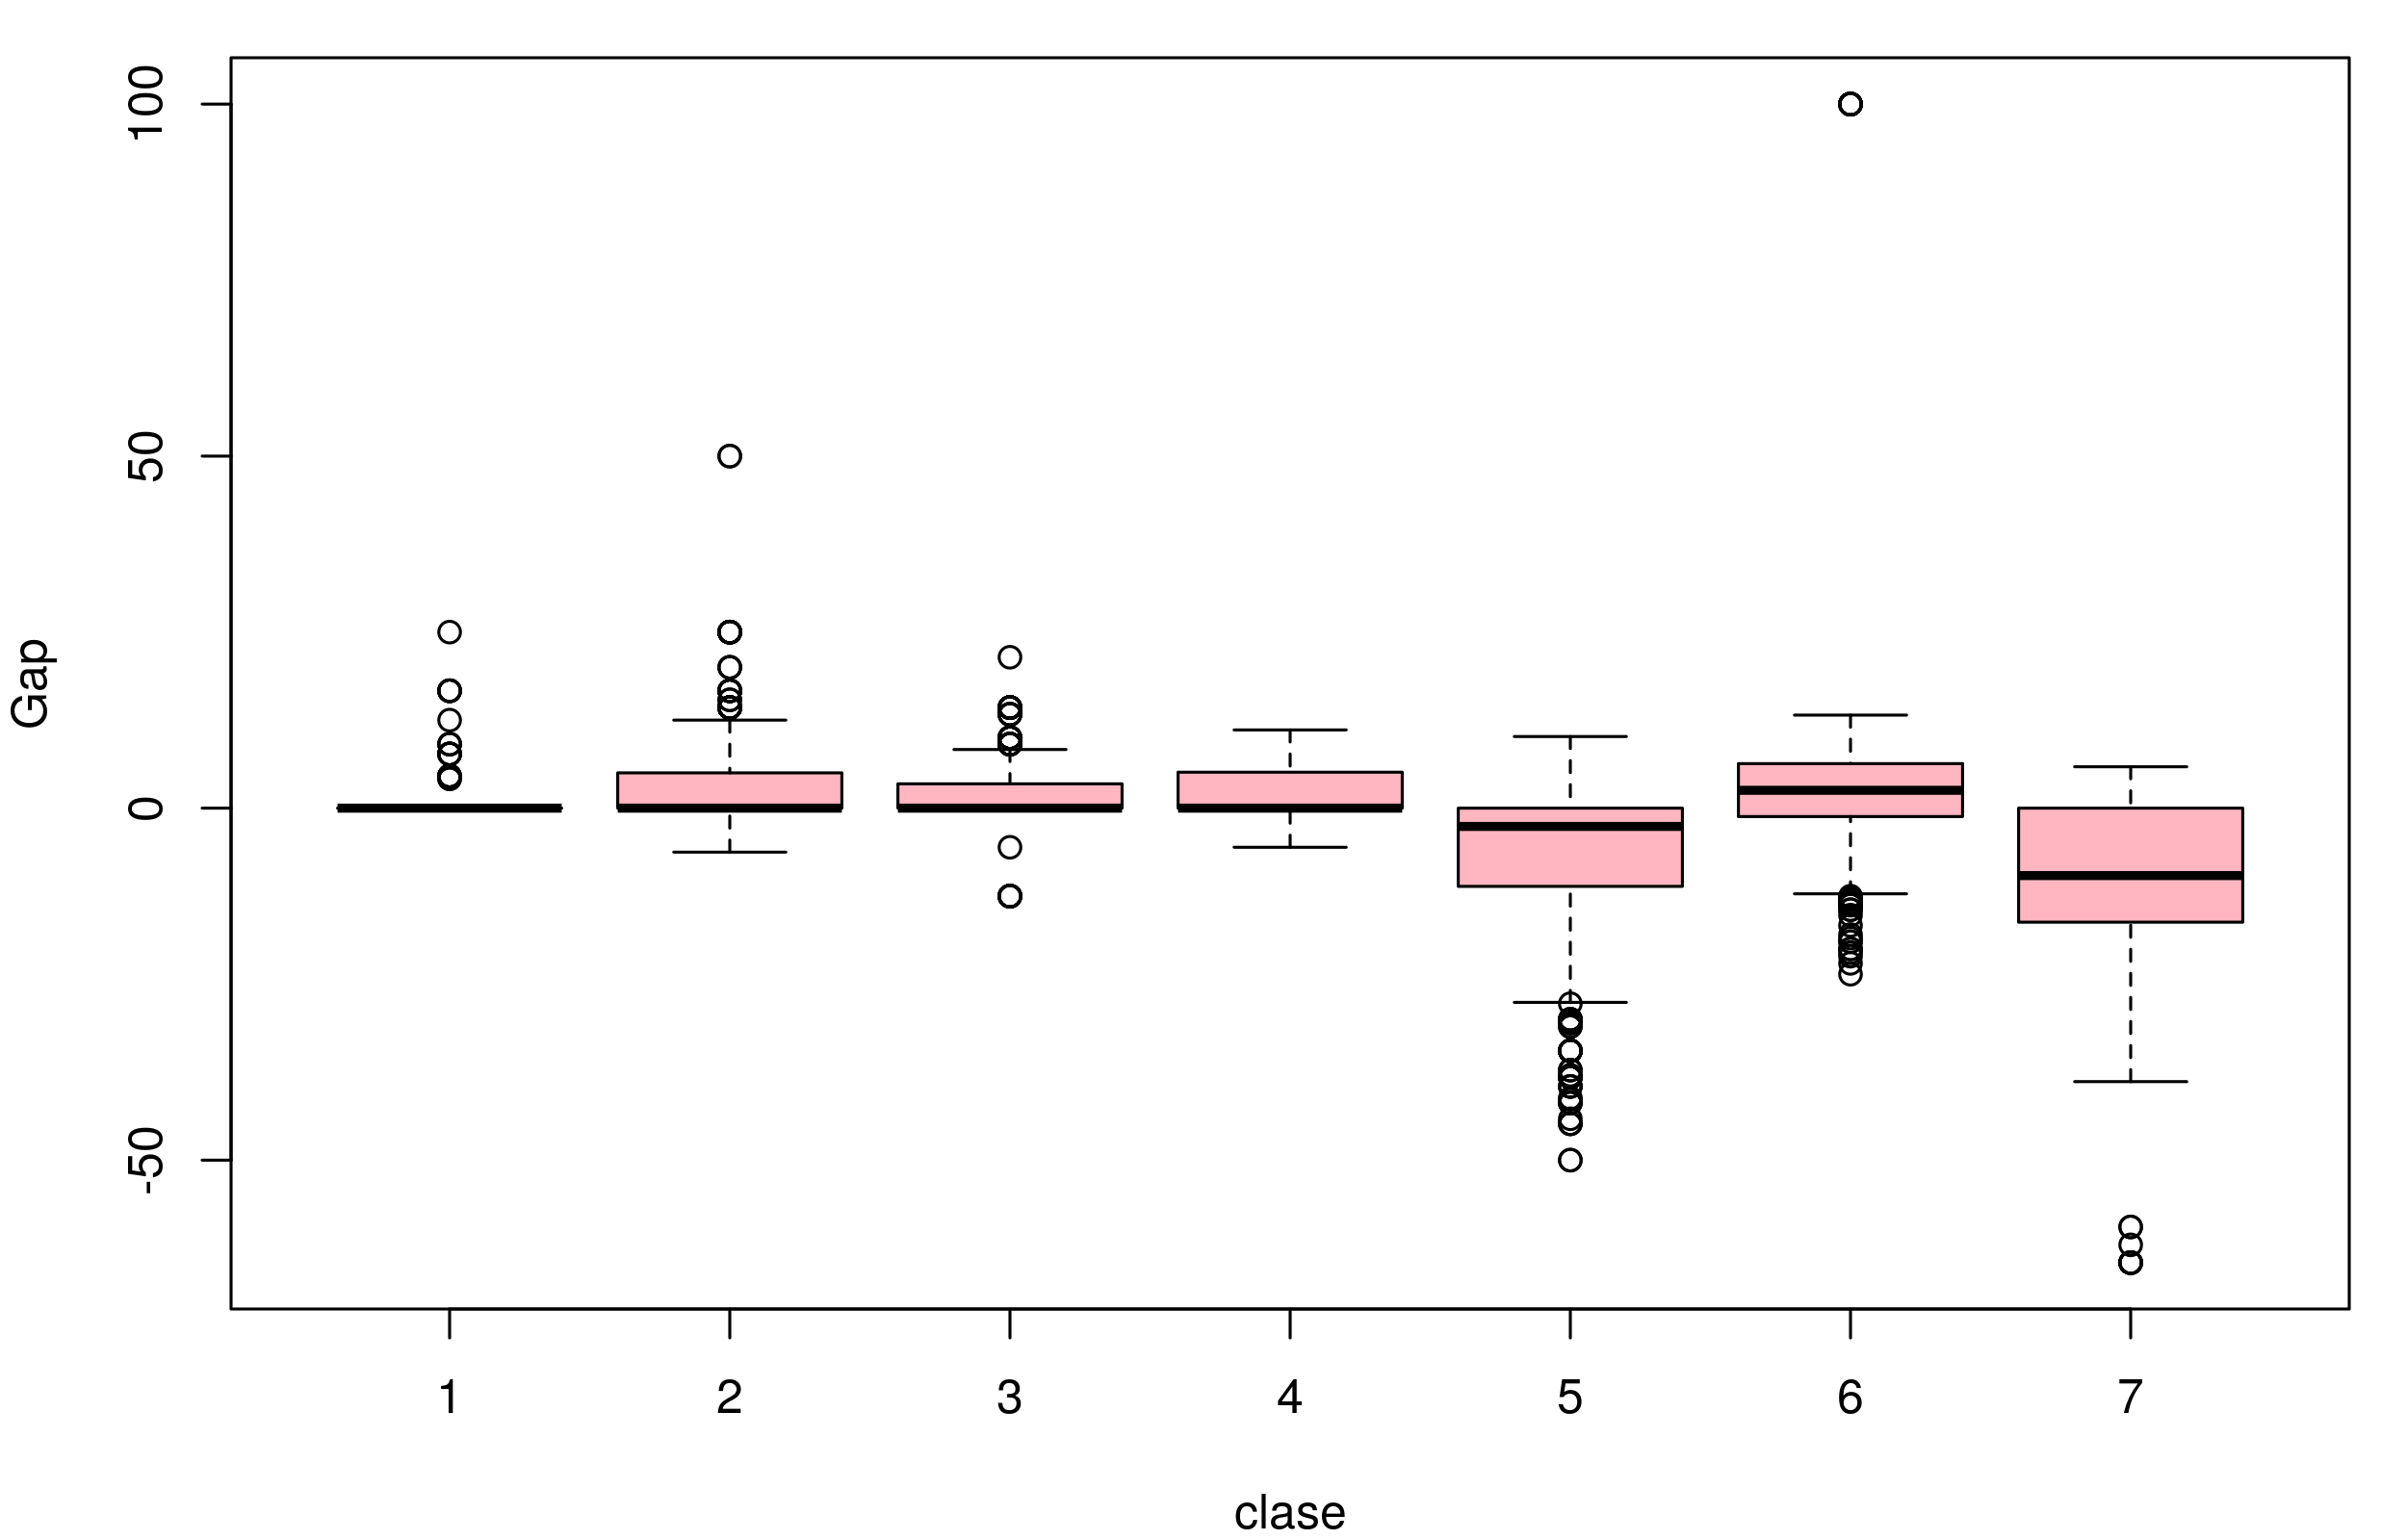
\includegraphics[width=0.8\textwidth]{box_gap21.png}
		\caption{Soluciones $s_{21}$}
	\end{subfigure}
	\caption{Gap para la función objetivo Max-Min separado por clase.}
	\label{boxob1}
\end{figure}

\begin{figure}
	\begin{subfigure}{\textwidth}
		\centering
		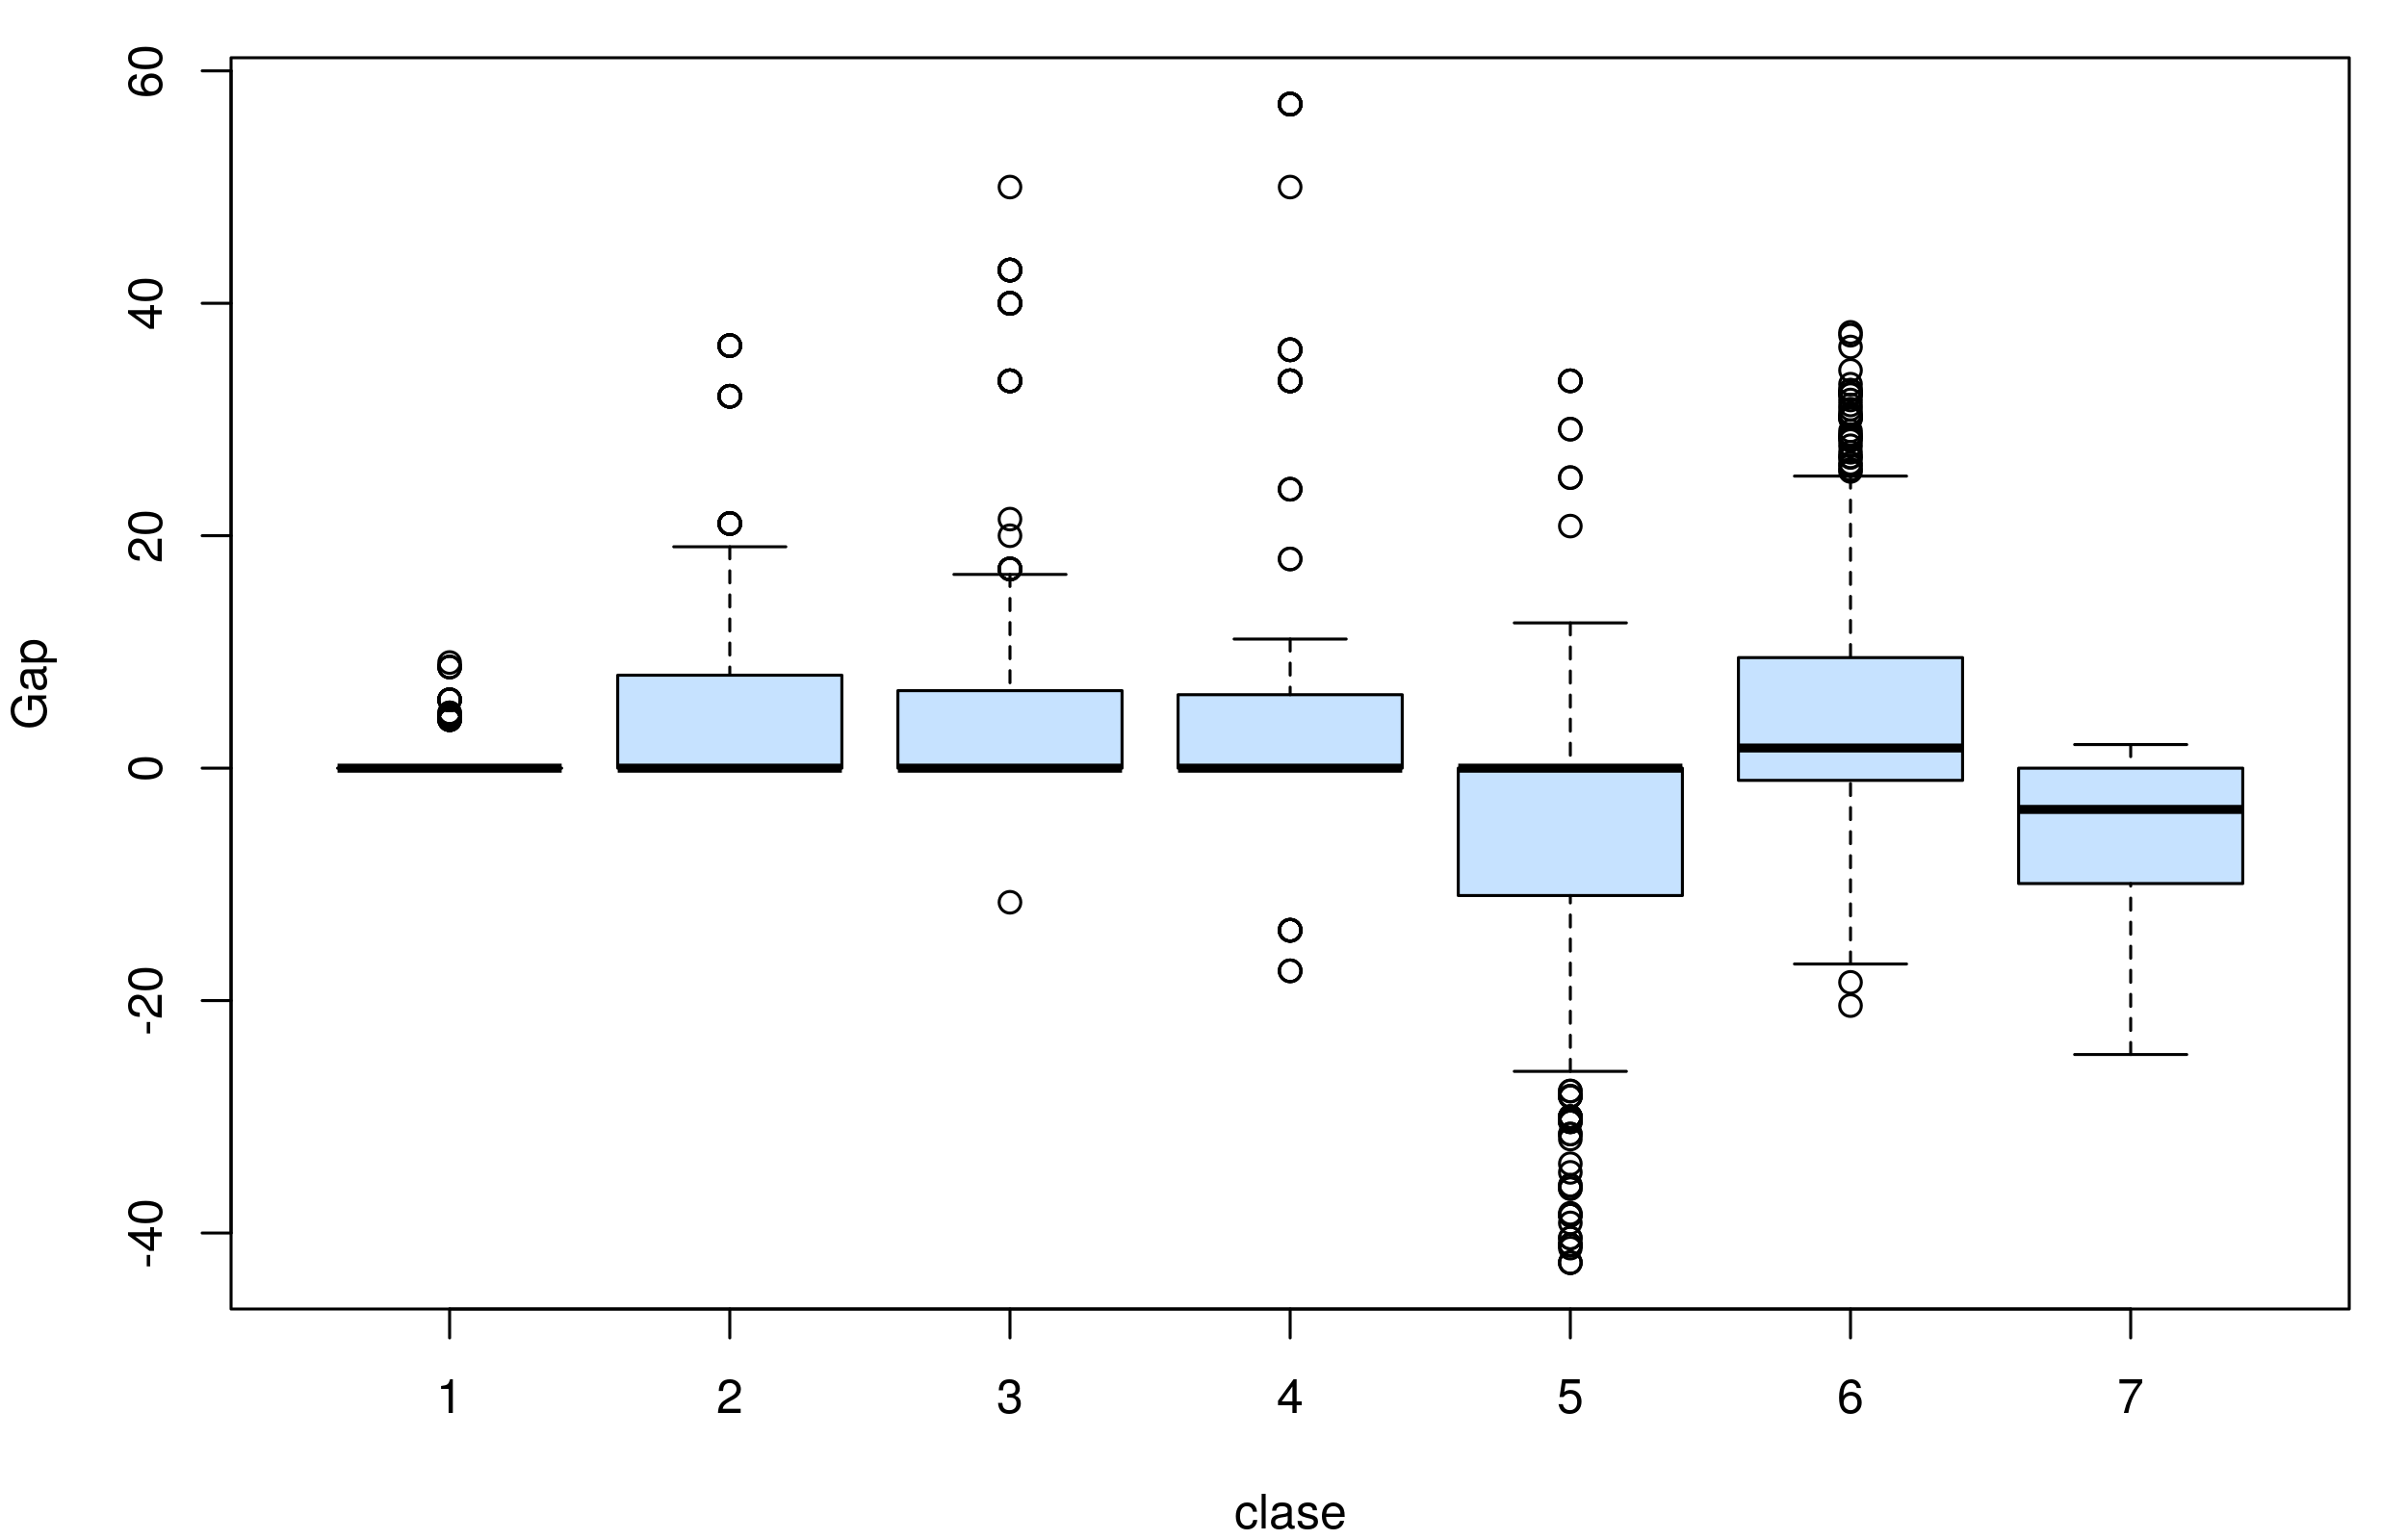
\includegraphics[width=0.8\textwidth]{box_gap2.png}
		\caption{Soluciones $s_2$}
	\end{subfigure}
	\begin{subfigure}{\textwidth}
		\centering
		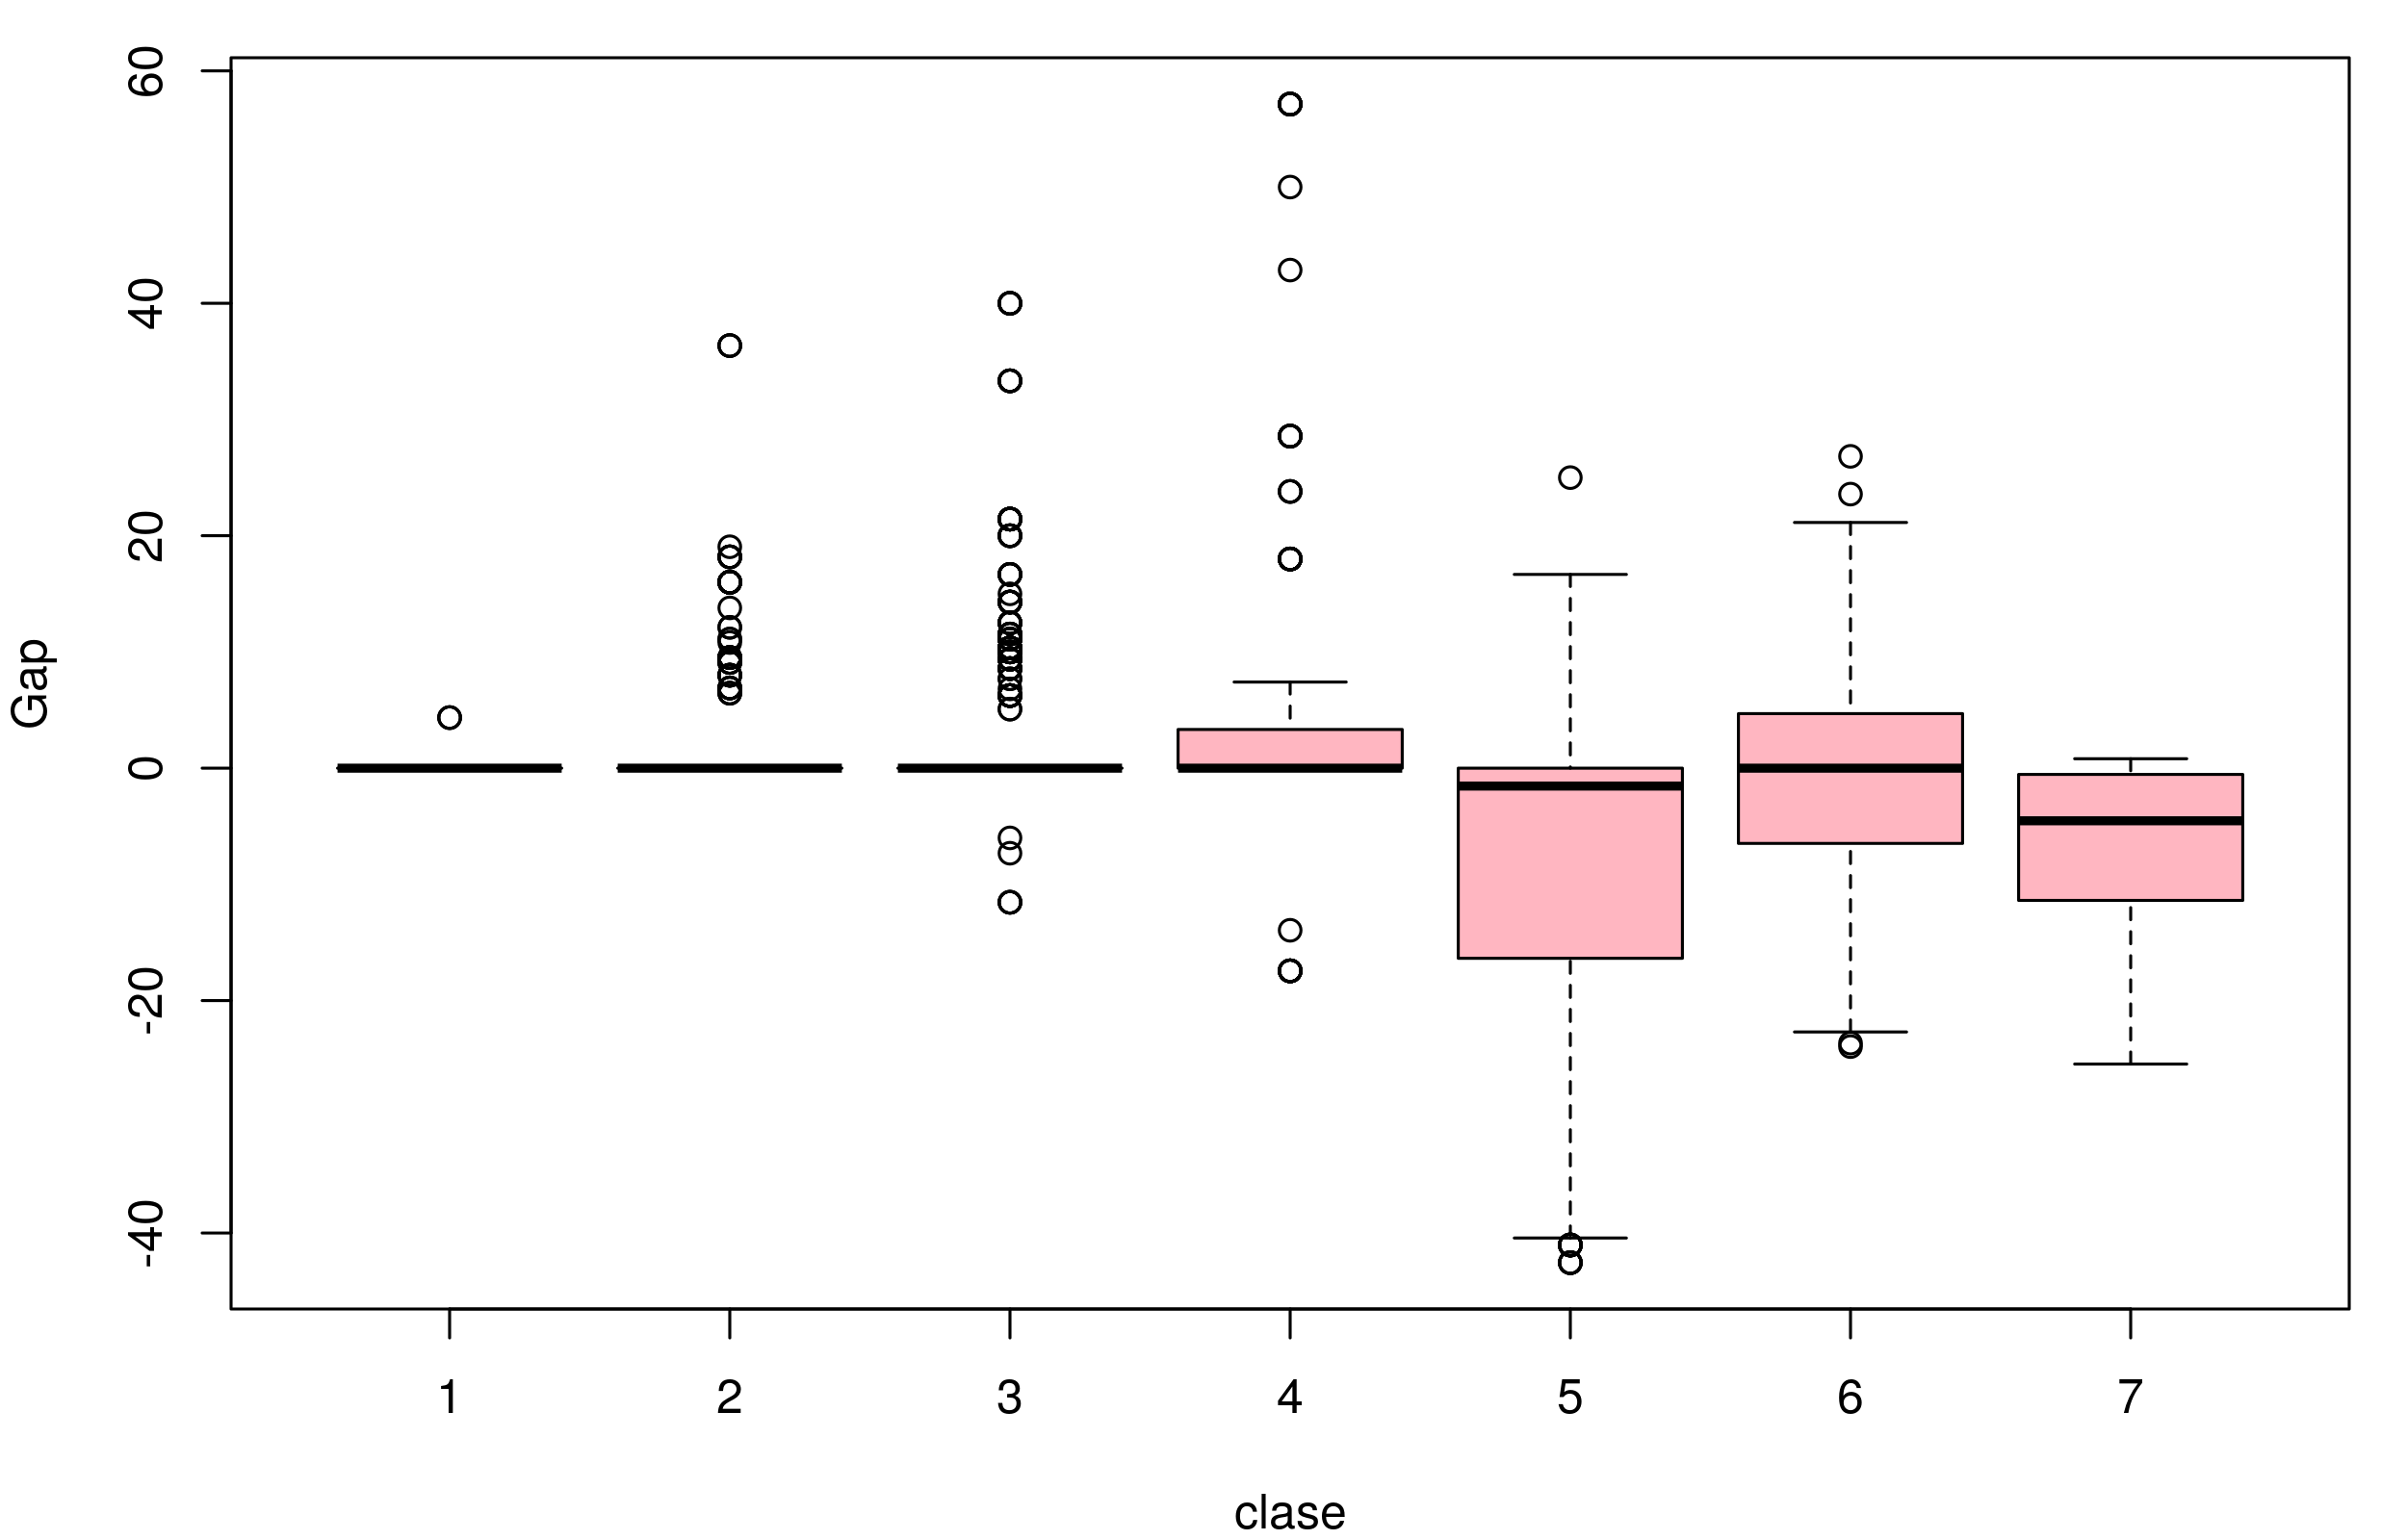
\includegraphics[width=0.8\textwidth]{box_gap12.png}
		\caption{Soluciones $s_{12}$}
	\end{subfigure}
	\caption{Gap para la función objetivo Min-Max separado por clase.}
	\label{boxob2}
\end{figure}

\begin{figure}
	\begin{subfigure}{\textwidth}
		\centering
		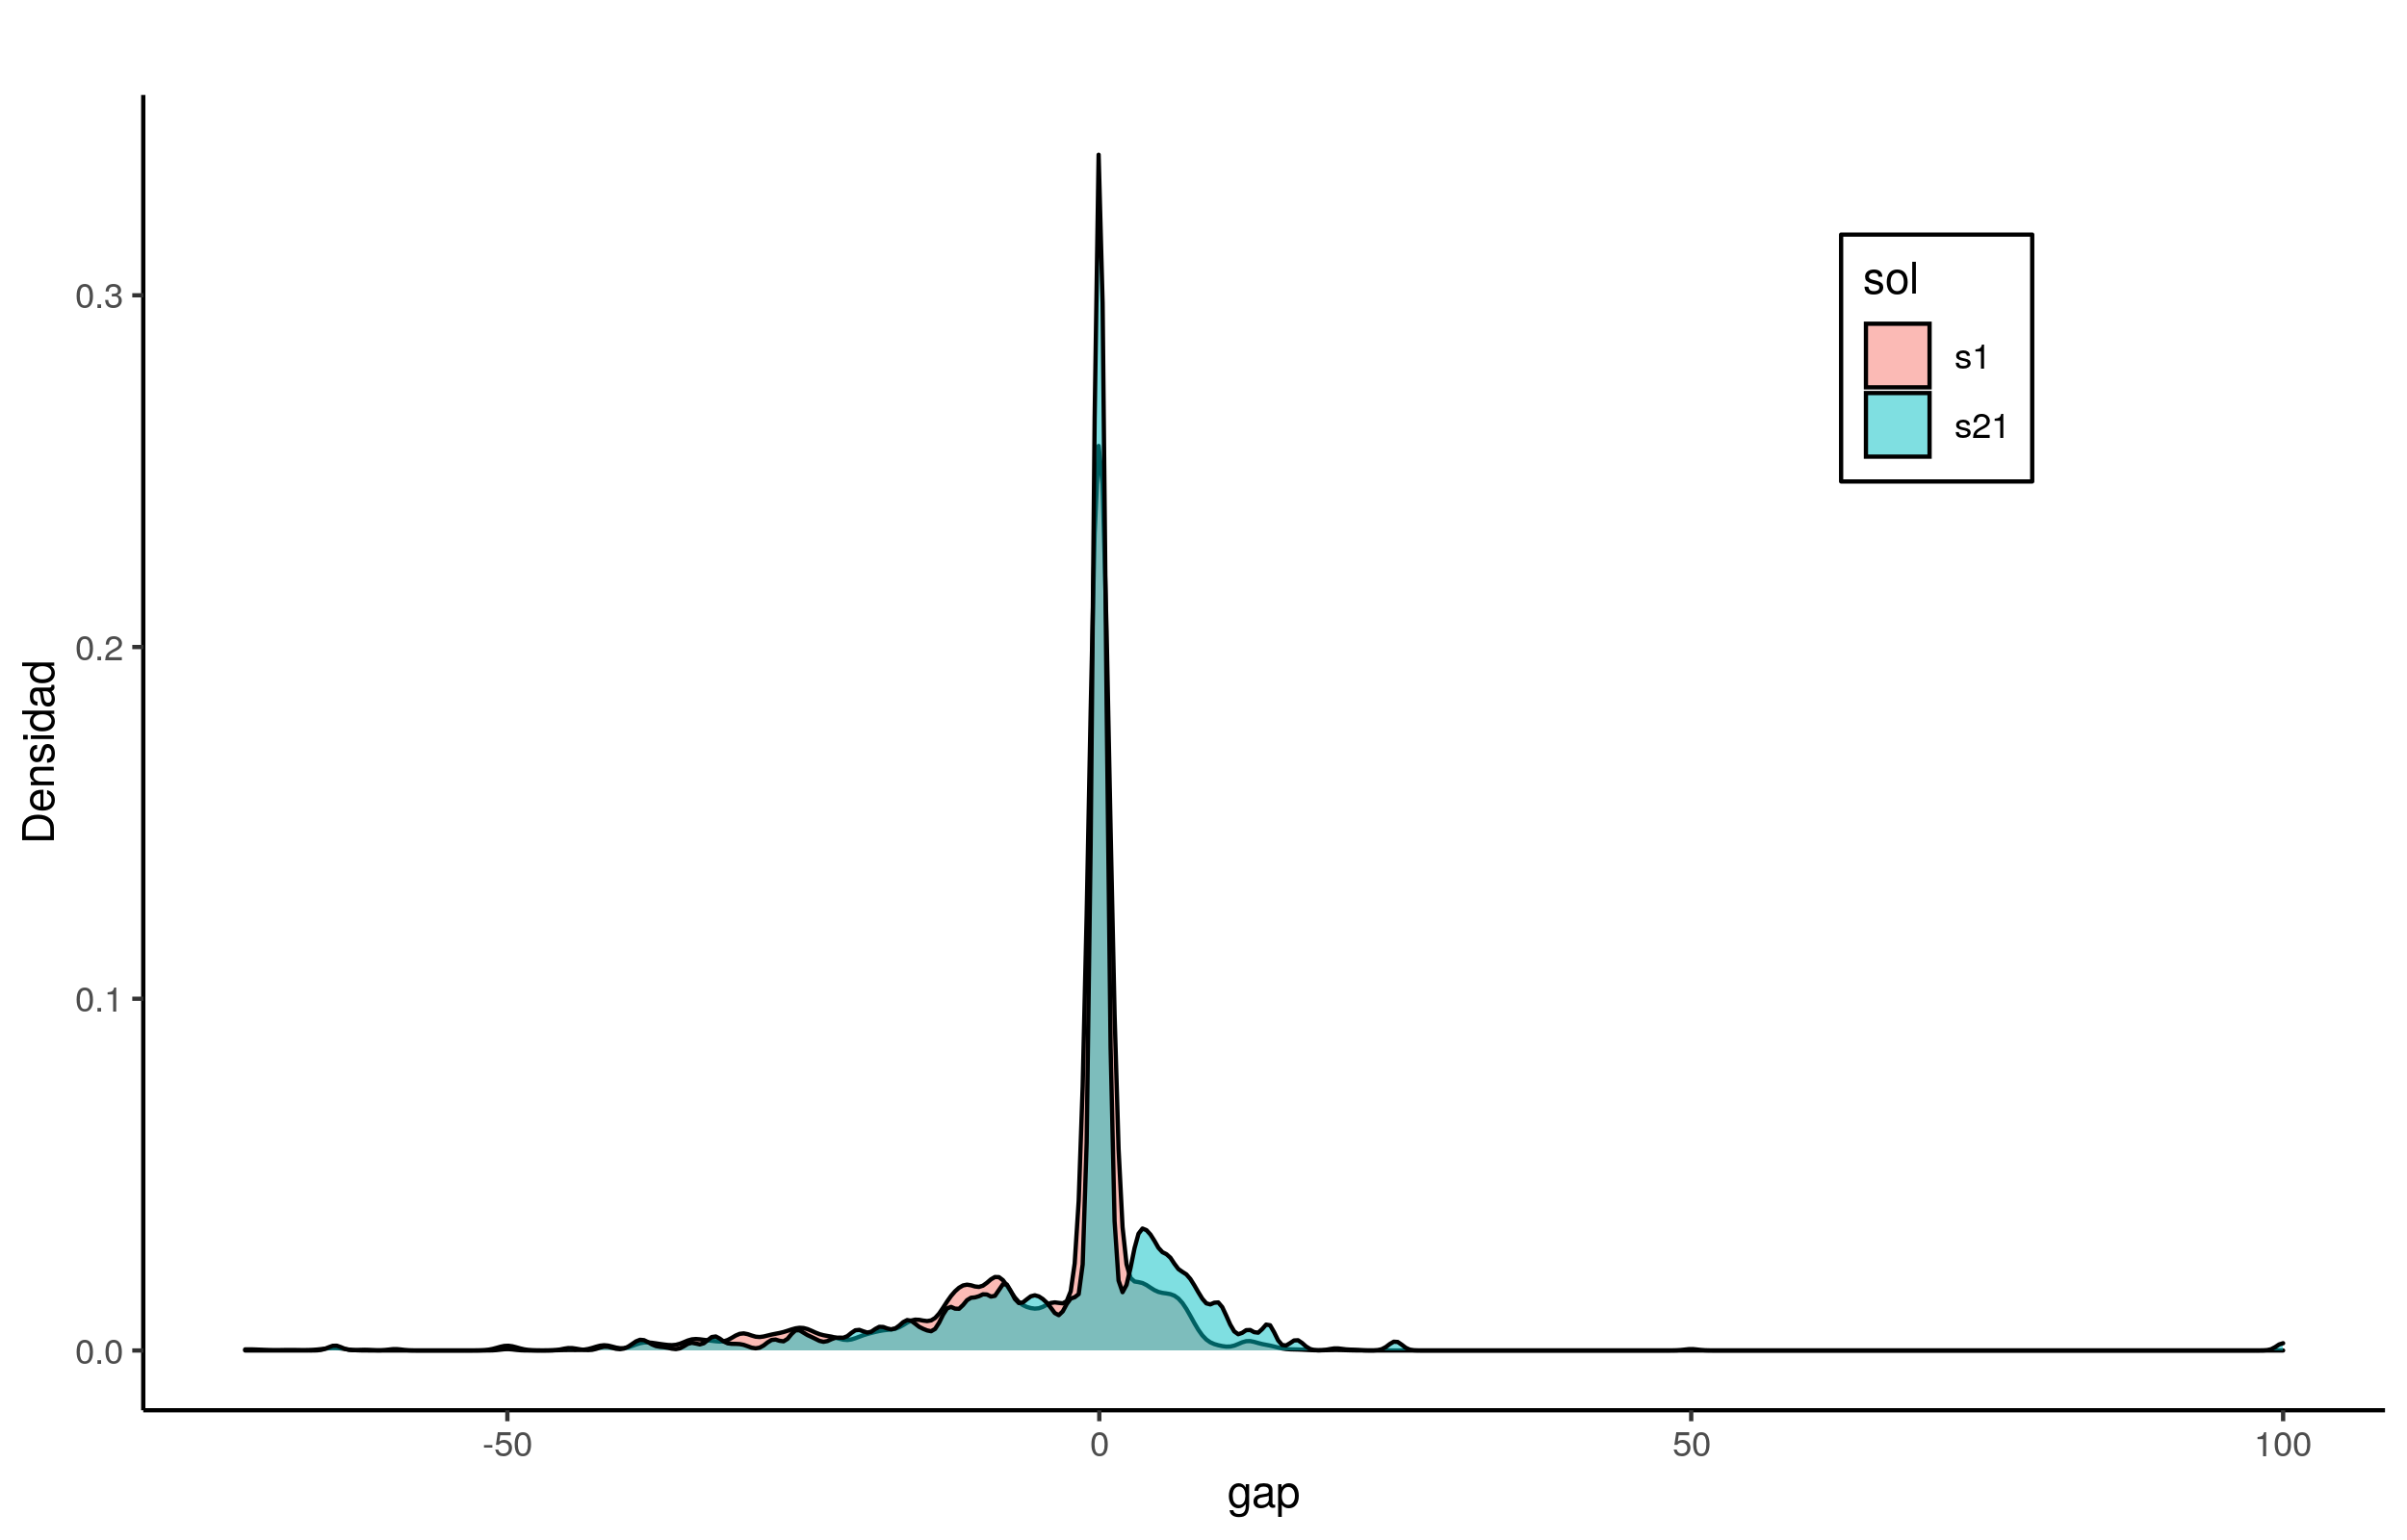
\includegraphics[width=0.8\textwidth]{histden_sols_ob1.png}
		\caption{Función objetivo Max-Min}
	\end{subfigure}
	\begin{subfigure}{\textwidth}
		\centering
		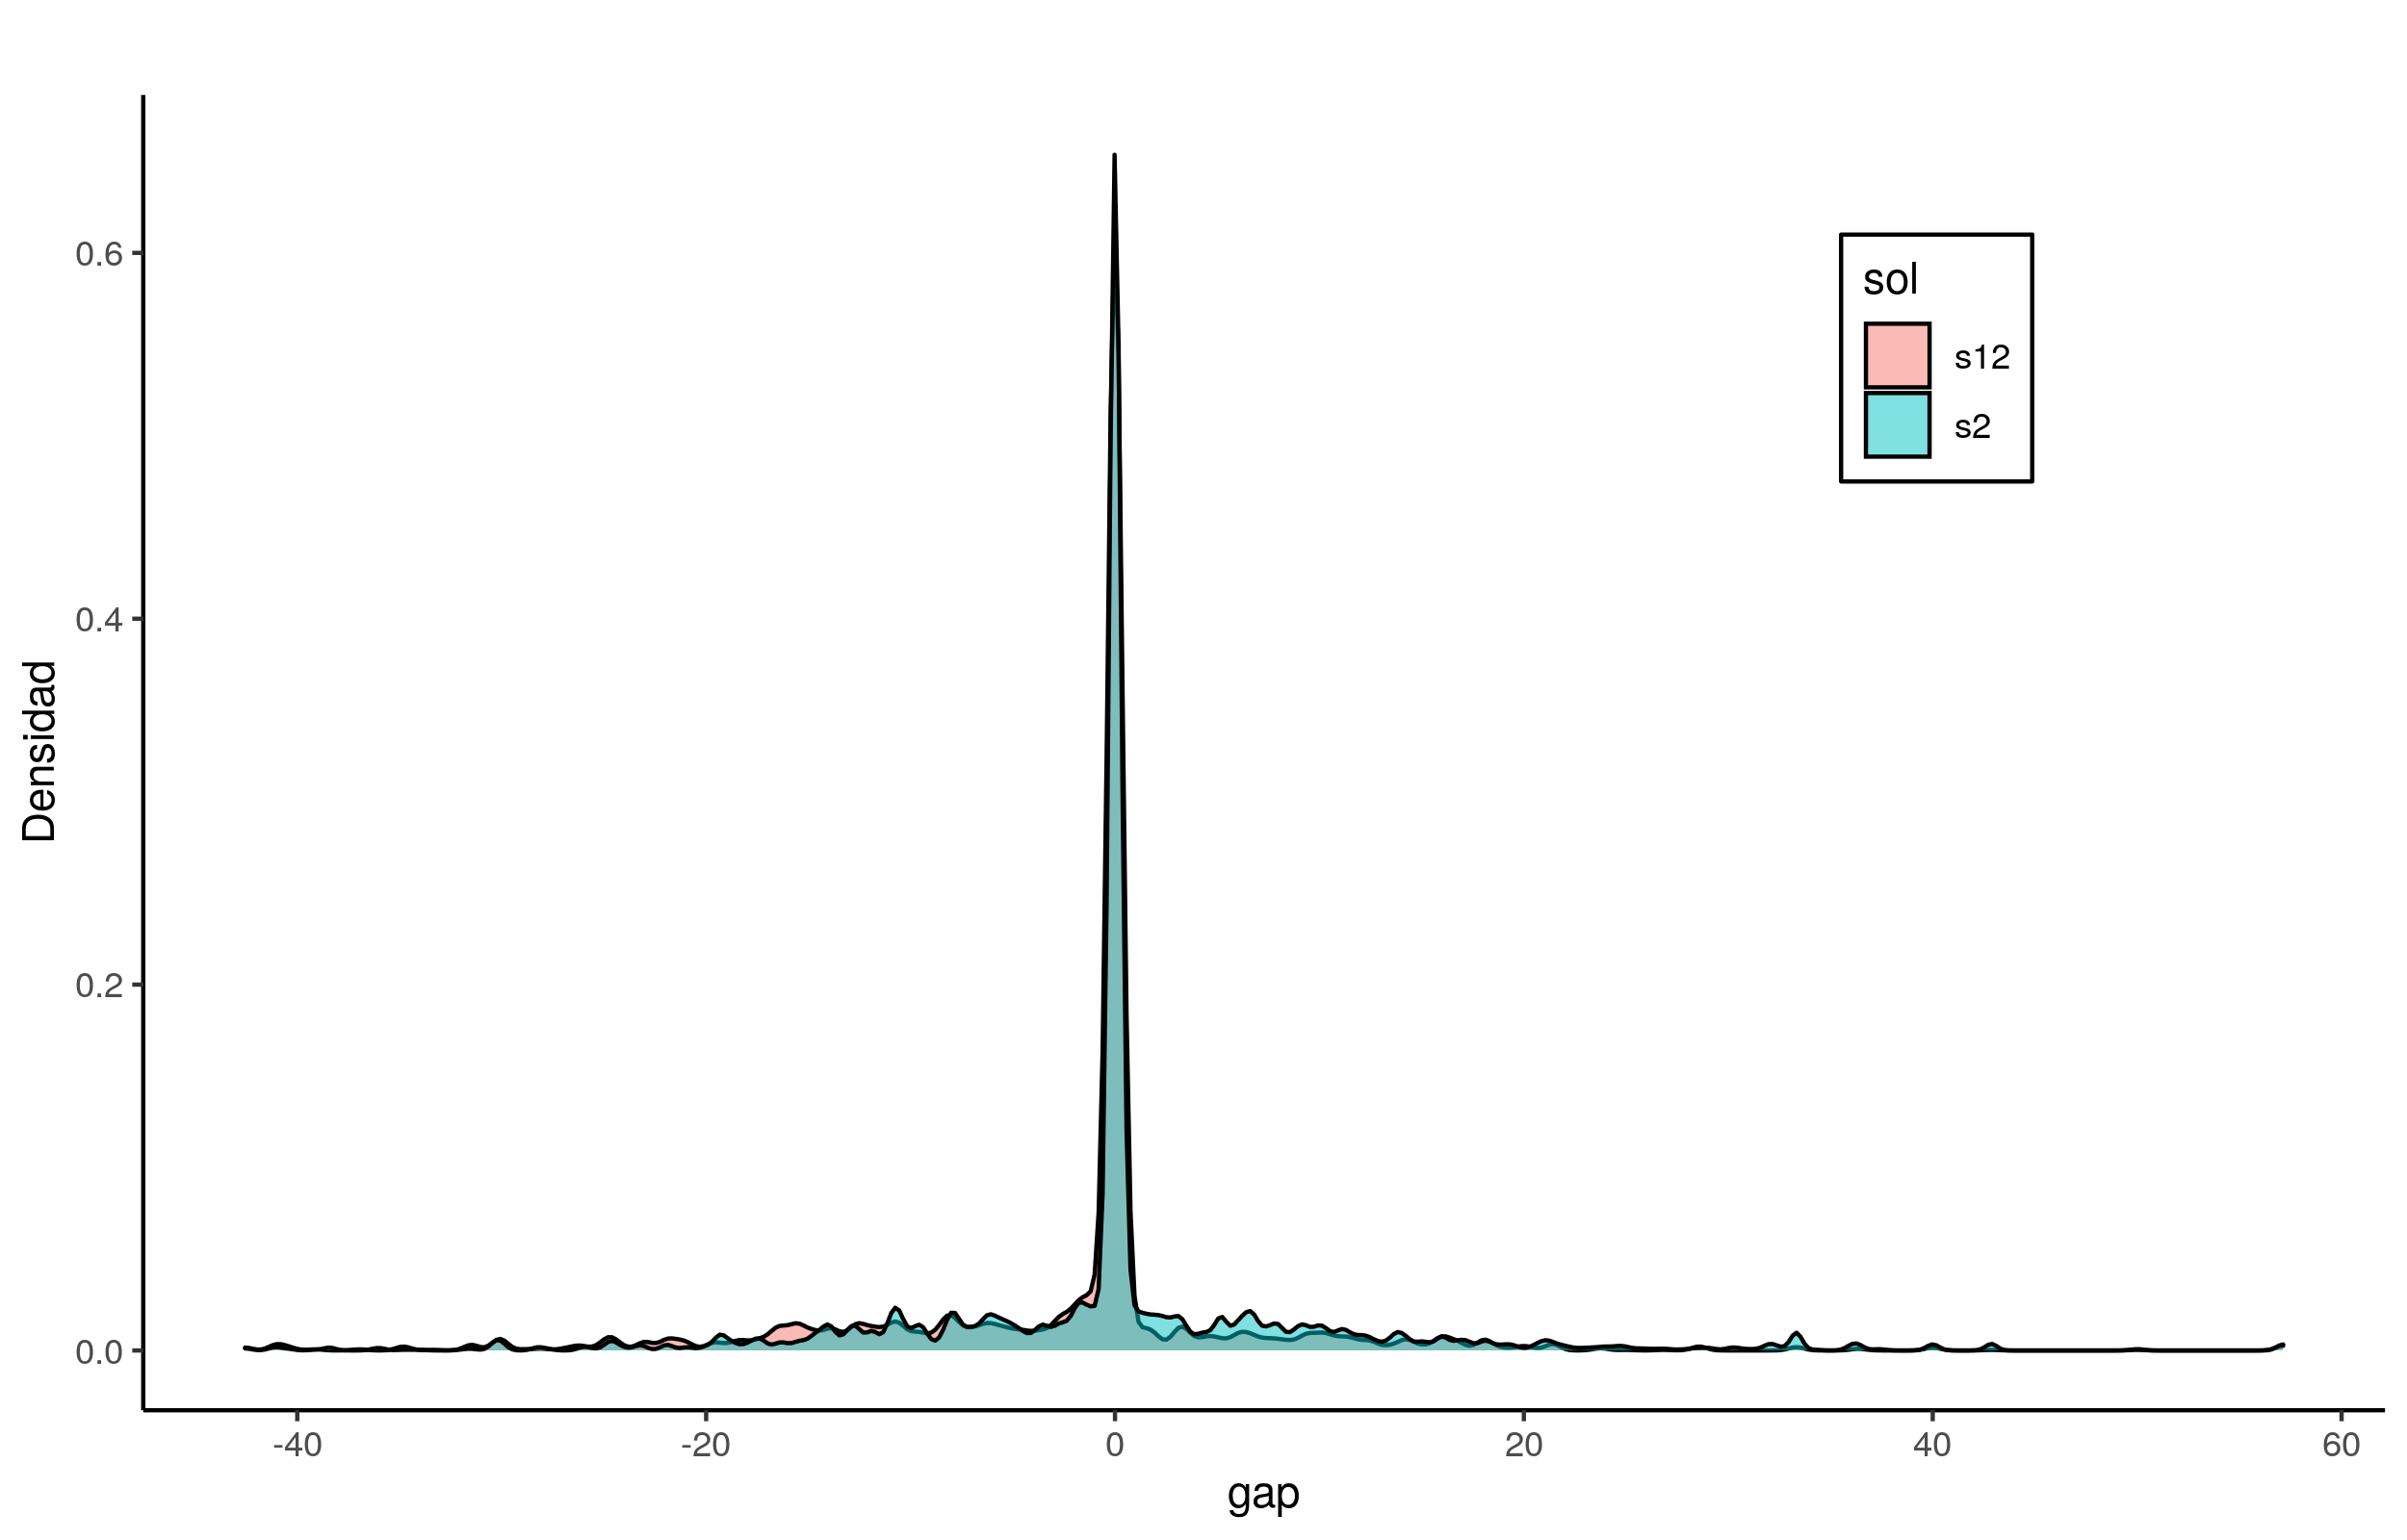
\includegraphics[width=0.8\textwidth]{histden_sols_ob2.png}
		\caption{Función objetivo Min-Max}
	\end{subfigure}
	\caption{Densidad del gap separado por función objetivo.}
	\label{densidad}
\end{figure}

Si se comparan directamente las medias de los conjuntos de datos se observa que la media del gap obtenido de las soluciones $s_1$ es -4.0173 mientras que la media del gap de las soluciones $s_{21}$ es -1.7953. En ambos casos es negativo lo que indica que, en promedio, las soluciones de la metaheurística son mejores que las del optimizador. Ya que la media de las soluciones $s_1$ es más pequeña, se podría decir que en promedio el modelo Max-Min mostró mejor desempeño. Al realizar el mismo análisis con las soluciones $s_2$ y $s_12$ los resultados obtenidos para las medias son 0.0313 y -1.9195, lo que permite concluir que en promedio nuevamente las soluciones del modelo Max-Min muestran mejores resultados. 

El análisis descriptivo muestra que sí hay ligeras diferencias entre los conjuntos. Sin embargo, no es suficiente para justificar si en general la diferencia será significativa o no. 


\section{Pruebas estadísticas}
\label{pe}

En esta sección se emplean pruebas estadísticas con el objetivo de justificar diferencias significativas en los resultados. Todas las pruebas usadas se realizan utilizando como apoyo el lenguaje de programación \textsc{R} \citep{r}. Como primer paso, es importante verificar si las muestras cumplen con la normalidad o no, ya que ayudará a determinar si deben usarse pruebas paramétricas o no paramétricas. 

\subsection{Normalidad}

Para determinar si los conjuntos de datos siguen una distribución normal se emplea la prueba de {\em Shapiro-Wilk}. Este test plantea la hipótesis nula de que la muestra proviene de una distribución normal, por lo tanto si el $p$-valor es menor que 0.05 se rechaza la hipótesis nula y se concluye que los datos no provienen de una distribución normal. Los resultados de los cuatro distintos conjuntos de datos indican que ninguno cumple con la normalidad por lo tanto sólo son utilizadas pruebas no paramétricas para analizar las diferencias entre los datos.

\subsection{Prueba de los rangos con signo de Wilcoxon}

Se resalta que el conjunto de instancias usadas para resolver ambos modelos es el mismo, por lo tanto se tienen datos {\em pareados}. La prueba de los rangos con signo de Wilcoxon permite analizar si hay diferencia entre las muestras pareadas. La hipótesis nula de la prueba es que la mediana de las diferencias de cada par es cero.

Al realizar la prueba para los dos pares de conjuntos de datos de estudio, el $p$-valor permite rechazar la hipótesis nula ya que es menor que el nivel de significancia. Se debe hacer énfasis en que existen varios pares en los cuales ambos datos son iguales, eso ocasiona lo que se conoce como {\em ties} o {\em ligaduras}. En este caso \texttt{wilcox.test()} devuelve un $p$-valor aproximado por lo que no se puede hacer una conclusión al respecto.  

%Por lo tanto se concluye que hay una diferencia estadísticamente significativa entre las soluciones de los conjuntos. 

Se optó por hacer una tercera prueba pareada en la que se consideran como datos las evaluaciones cruzadas, es decir el gap obtenido de las soluciones $s_{12}$ y $s_{21}$. El resultado del $p$-valor en este panorama no permite rechazar la hipótesis nula. Sin embargo, sucede lo mismo que en los casos anteriores, hay pares de datos iguales que generan ligaduras por lo que tampoco se puede concluir con seguridad un resultado. %concluye que no hay suficiente evidencia estadística que indique una diferencia entre los resultados de los dos modelos.

%\subsection{Prueba de $\chi^2$}



\section{Conclusiones}
\label{conclusiones}

El empleo de la prueba para muestras pareadas no permite hacer conclusiones respecto a los datos ya que los datos generan ligaduras. Como trabajo a futuro se puede implementar la estrategia descrita por \cite{degroot2012} para tratar con estos casos. Otro punto a resaltar en esta prueba es que de cada instancia hay diez replicas por lo que podría haber diferencias en el resultado del $p$-valor si los pares de conjuntos de datos se consideran de forma diferente. Una estrategia a implementar es reducir el tamaño de las muestras al usar únicamente los mejores resultados obtenidos para cada una de las instancias.
%permitió concluir que hay una diferencia significativa entre los datos. Sin embargo, no es posible concluir sobre cuál de los dos modelos proporciona mejores soluciones. 


%% The Appendices part is started with the command \appendix;
%% appendix sections are then done as normal sections
%% \appendix

%% \section{}
%% \label{}

%% If you have bibdatabase file and want bibtex to generate the
%% bibitems, please use
%%
  \bibliographystyle{elsarticle-harv}
  %\bibliographystyle{elsarticle-num} 
  \bibliography{biblio}

%% else use the following coding to input the bibitems directly in the
%% TeX file.

%\begin{thebibliography}{00}
%
%%% \bibitem[Author(year)]{label}
%%% Text of bibliographic item
%
%\bibitem[ ()]{}

%\end{thebibliography}
\end{document}

\endinput
%%
%% End of file `elsarticle-template-harv.tex'.
